% Create a Table of Contents in Beamer
\documentclass[10pt,t]{beamer}
% Theme choice:
\usetheme{Singapore}
\useoutertheme{sidebar}
\usecolortheme{seahorse}
\setbeamercolor{titlelike}{bg=white}
\setbeamercolor{frametitle}{bg=white}
%\setbeamertemplate{frametitle}[default][left]
\setbeamertemplate{navigation symbols}{}

\usepackage{graphicx}
\usepackage{amsmath}
\usepackage{amsfonts}
\usepackage{amssymb}
\usepackage{amsthm}
\usepackage[normalem]{ulem}

\newcommand\tab[1][1cm]{\hspace*{#1}}

% Title page details: 
\title{Chapter 2: Regression for binary outcomes} 
\author{Taylor Okonek \& Charlie Wolock}
\date{\today}



\begin{document}
	% Title page frame
	\begin{frame}
	\titlepage 
\end{frame}

\begin{frame}{Learning objectives}
	By the end of Chapter 2, you should be able to: 
	\begin{itemize}
		\item Distinguish between probability and odds and know how to calculate each in \texttt{R}
		\item Describe the measures of association used for binary outcomes and exposures of interest
		\item Formulate a regression model, given a scientific or statistical question about a binary outcome
		\item Interpret the coefficients (along with confidence intervals and p-values) of a regression model for a binary outcome
		\item Describe how (and why) logistic regression interpretation changes when we have data from a case-control study
		\item Use \texttt{R} to fit a logistic regression model and produce supporting figures/tables
	\end{itemize}
\end{frame}

% Outline frame
\begin{frame}{Outline}
\tableofcontents
\end{frame}

\AtBeginSection[ ]
{
\begin{frame}{Outline}
\tableofcontents[currentsection]
\end{frame}
}

% Presentation structure
\section{Binary outcomes}

% quantitative outcomes from ch1
\begin{frame}{Recall: Variable type}
	In Chapter 1, we asked scientific questions involving quantitative outcomes: those that have a fundamentally numeric quality: 
	\\~\
	
	\begin{itemize}
		\item Our primary outcome of interest was \textcolor{blue}{birthweight}
		\item We also saw brief examples involving FEV, 100m dash times, dental patient pain ratings
	\end{itemize}
\end{frame}

% binary variable examples
\begin{frame}{Recall: Variable type}
Binary variables are a type of \textcolor{blue}{categorical} variable with two possible categories. We often implicitly think of them in a 0-1 sense, but they often don't have actual numeric value. 
\\~\

Examples we often see in biomedical research: 
\begin{itemize}
	\item Type I diabetes (presence/absence)
	\item Surgery complications (occurred/did not occur)
	\item Smoking (yes/no)
	\item Mortality prior to age 5 (occurred/did not occur)
	\item COVID status (positive/negative)
\end{itemize}
\end{frame}

% binary variable scientific questions
\begin{frame}{Scientific questions about binary variables}
	Questions we could ask about these variables include
	\begin{itemize}
		\item Are variants in the HLA-DRB1 gene associated with \textcolor{blue}{Type I diabetes}? 
		\item Are \textcolor{blue}{surgery complications} after upper endoscopy associated with who (anesthesiologist vs nurse) performed the sedation?
		\item Is the use of e-cigarettes associated with \textcolor{blue}{smoking}?
		\item \textcolor{red}{Insert question from Taylor here}
		\item Is Vitamin D intake associated with the risk of \textcolor{blue}{testing positive for COVID}?
	\end{itemize}
\end{frame}

\begin{frame}{Scientific questions about binary variables}
	One specific question that has been the subject of much study is 
	\begin{itemize}
		\item Is Type A behavior associated with risk of \textcolor{blue}{coronary heart disease} (CHD)?
	\end{itemize}
	\vspace{0.7cm}
	Type A behavior is a concept that was developed by cardiologists in the 1950s, and is characterized by being competitive, ambitious, work-driven, and time-conscious. The doctors who identified this ``personality type" thought it might be associated with the risk of CHD, and many studies investigated this association. 
\end{frame}

\begin{frame}{The WCGS Study}
	The Western Collaborative Group Study (WCGS) was designed in order to investigate a possible link between Type A behavior and CHD, and to develop a \textcolor{blue}{risk prediction} framework to select patients for intervention in order to decrease risk of CHD. 
	\\ ~\ 
	
	\textbf{Study description}: 3154 men aged 39-59 in California with no CHD history were enrolled in 1960 and 1961, subjected to a medical examination and history, and re-examined annually for interim cardiovascular history. The primary outcome was angina pectoris (chest pain due to heart disease). 
	\\ ~\
	
	\textcolor{blue}{\textbf{Exercise:}} What study design is this? \pause
	\\~\
	
	\textcolor{blue}{\textbf{Answer:}} Prospective cohort study
\end{frame}

\begin{frame}{Recall: summarizing a binary variable}
	Let's think about Type A behavior  and CHD. 
	\\ ~\ 
	
	We can talk about the \textcolor{blue}{probability} of experiencing CHD among those with Type A behavior ($p_A$) and the probability of experiencing CHD among those without Type A behavior ($p_B$).
	\begin{itemize}
		\item Generally, ``probability," ``risk," ``proportion" refer to the same quantity.
	\end{itemize}
	\textcolor{blue}{Odds} are defined as $\frac{p}{1-p}$.
	\begin{itemize}
		\item Odds of CHD with Type A behavior: $\frac{p_A}{1-p_A}$
		\item Odds of CHD without Type A behavior: $\frac{p_B}{1-p_B}$
	\end{itemize}
\end{frame}

\begin{frame}{Recall: summarizing a binary variable}
Probability:
\begin{itemize}
	\item Takes values in $[0,1]$.
	\item Generally more intuitive than odds. 
	\item In some study designs, are impossible to estimate! (More on this later.)
\end{itemize}
Odds:
\begin{itemize}
	\item Take values in $(0,\infty)$.
	\item Are less intuitive for most people (unless you do a lot of betting).
	\item Can be estimated from most common biomedical study designs. 
\end{itemize}
\end{frame}

\begin{frame}{Measures of association}
	We can now describe the \textcolor{blue}{probability} or \textcolor{blue}{odds} of having CHD among those with Type A behavior and those without. 
	\\ ~\
	
	\textbf{Scientific question:} Is exhibiting Type A behavior \textcolor{red}{associated} with CHD? 
	\\ ~\
	
	In order to do statistics, we need to clarify what \textcolor{red}{associated} means for binary variables.
\end{frame}

\begin{frame}{Measures of association}
Equal probabilities: If $p_m = p_w$, then
	\begin{itemize}
		\item[] $p_A - p_B = 0$ (\textcolor{red}{risk difference}) \quad \quad \quad $\frac{p_A}{p_B} = 1$ (\textcolor{red}{relative risk})
	\end{itemize}
	\vspace{0.8cm}
Equal odds: If $\frac{p_A}{1-p_A} = \frac{p_B}{1-p_B}$, then
	\begin{itemize}
		\item[] $\frac{\frac{p_A}{1-p_A}}{\frac{p_B}{1-p_B}}=1$ (\textcolor{red}{odds ratio})
	\end{itemize}
\vspace{0.8cm}
These are the three most common measures of association for binary outcomes. 
\end{frame}

\begin{frame}{Measures of association}
When we are approaching a scientific question about association, we need to think about
\begin{itemize}
	\item \textcolor{blue}{Summary measure:} Probability or odds
	\item \textcolor{red}{Contrast:} Difference or ratio
\end{itemize}
\vspace{0.5cm}
In our running example:
\begin{itemize}
	\item Is there a \textcolor{red}{difference} in the \textcolor{blue}{probability} of CHD between people with Type A behavior and those without? \pause
	\item Is the \textcolor{red}{ratio} of \textcolor{blue}{probabilities} of CHD comparing people with and without Type A behavior equal to 1? \pause
	\item Is the \textcolor{red}{ratio} of \textcolor{blue}{odds} of CHD comparing people with and without a Type A behavior equal to 1? \pause
\end{itemize}
\end{frame}

\begin{frame}{Moving toward statistical inference}
	The full process:
	\begin{enumerate}
		\item Ask a scientific question: Is Type A behavior associated with CHD?\pause
		\item Translate to a statistical question: Is there a \textcolor{red}{difference} in the \textcolor{blue}{probability} of CHD between people with Type A behavior and those without? \pause
		\item Define a parameter: In this case, risk difference \pause
		\item Take a sample: Think back to what we know about study design! \pause
		\item Perform inference: 
		\begin{itemize}
			\item Calculate a statistic based on our sample
			\item Quantify uncertainty: confidence interval
			\item Perform a hypothesis test: p-value
		\end{itemize}
	\end{enumerate}
\end{frame}



%% Linear regression
\section{Linear regression with binary outcomes}
\begin{frame}
	\frametitle{SECTION 2: LINEAR REGRESSION WITH BINARY OUTCOMES}
	
	% Learning objectives
	By the end of this section, you should be able to:
	\begin{itemize}
		\item Interpret linear regression coefficients when the outcome $Y$ is binary
		\item Write a summary of results from a linear regression analysis with a binary outcome
		\item List at least one advantage and one disadvantage of using linear regression with a binary outcome
	\end{itemize}
\end{frame}
\begin{frame}
	\frametitle{Simple linear regression with a binary outcome}
	Can we use linear regression to look at the association between an exposure and a binary outcome? Yes!
	\\ ~\
	
	A simple linear regression model: $E[Y \mid X] = \beta_0 + \beta_1 X$.
	\begin{footnotesize}
		\begin{itemize}
			\item Recall: $E[Y \mid X]$ is the \textcolor{blue}{\textit{expected value}} (average) of $Y$ given $X$ 
		\end{itemize}
	\end{footnotesize}
	\pause
	What's the average of a binary variable $Y$? \pause \textit{It's the probability that $Y$ equals 1!} $\left(\text{i.e., } E[Y] = \text{P}(Y=1)\right)$ \pause
	
	\begin{itemize} \itemsep +12pt
		\item[] $Y = \{ 0, 0, 1, 0, 1, 1, 0, 0, 1, 1 \}$ \pause
		\item[] $\bar{Y} = \frac{0 + 0 + 1 + 0 + 1 + 1 + 0 + 0 + 1 + 1}{10} = \frac{1}{2}$ \pause
		\item[] $\hat{p} = \hat{\text{P}}(Y=1) = \frac{5}{10} = \frac{1}{2} $
	\end{itemize}
\end{frame}

\begin{frame}
	\frametitle{Simple linear regression with binary outcomes}
	\textbf{Discuss with your neighbor:} 
	\\ ~\ 
	
	% recall activity
	Suppose we fit the simple linear regression model $$E[Y \mid X] = \beta_0 + \beta_1 X,$$ where our outcome $Y$ is binary.
	
	What is the interpretation for the coefficients in this model?
	
	\begin{enumerate}
			\item $\beta_0$
			\item $\beta_1$
		\end{enumerate} 
\end{frame}

\begin{frame}
	\frametitle{Simple linear regression with binary outcomes}
	\textbf{Discuss with your neighbor:} 
	\\ ~\ 
	
	% recall activity
	Suppose we fit the simple linear regression model $$E[Y \mid X] = \beta_0 + \beta_1 X,$$ where our outcome $Y$ is binary.
	
	What is the interpretation for the coefficients in this model?
	
	\begin{enumerate}
		\item $\beta_0$: probability $Y = 1$ among those with $X = 0$
		\item $\beta_1$: difference in probability that $Y = 1$ comparing those with $X = 1$ and those with $X = 0$ \footnotesize{(\textit{Nothing more than our usual difference in means!})}
	\end{enumerate} 
\end{frame}

% linear regression: diabetes vs sex
\begin{frame}
	\frametitle{Simple linear regression: Type A personality and CHD}
	\vspace{-0.5cm}
	In our \texttt{wcgs} dataset, \texttt{chd} is a binary variable indicating CHD over follow-up, and \texttt{tabp} is a binary variable indicating Type A behavior. 
	\\ ~\
	
	We can fit the linear regression model $E[\texttt{chd} \mid \texttt{tabp}] = \beta_0 + \beta_1\texttt{tabp} $.
	
	How do we interpret the regression coefficients? \vspace{-0.2cm}
	
	\begin{itemize}
		\item \color{blue} $\beta_0$: \pause the probability of CHD among those without Type A behavior \pause \color{black}\vspace{-0.2cm}
		\item[] \ \ \begin{scriptsize} (the average value of \texttt{chd} among those with $\texttt{tabp} = 0$) \end{scriptsize} \pause
		\item \color{blue} $\beta_1$: \pause the difference in probability of CHD between those with and without Type A behavior \pause \color{black} \vspace{-0.2cm}
		\item[] \ \ \begin{scriptsize}(the difference in average value of \texttt{chd} between \texttt{tabp} = 1 and \texttt{tabp} = 0 groups) \pause \end{scriptsize}
	\end{itemize}
	
	\vspace{-0.2cm}
	To answer our statistical question \begin{small}\textit{(is there a difference in probability of CHD between Type A and others?)}\end{small} we just need to look at $\beta_1$!
\end{frame}

\begin{frame}{Simple linear regression example}
	\vspace{-0.8cm}
	We'll leave the CHD and Type A behavior analyses for your homework! Another binary variable in our dataset is \texttt{arcus}, which is an indicator of whether or not the subject had \textit{arcus senilis} (a visible ring around the cornea that indicates high cholesterol). Here's \texttt{R} output from fitting the model $E[\texttt{chd} \mid \texttt{arcus}] = \beta_0 + \beta_1 \texttt{arcus}$:
	
	\begin{center}
		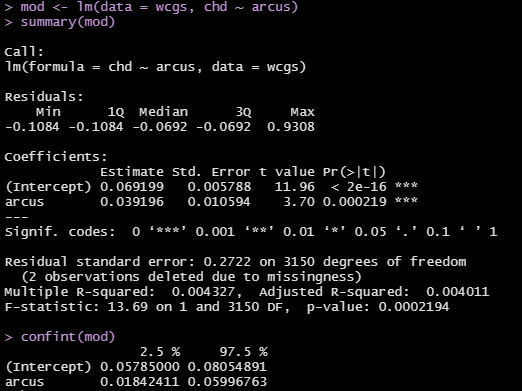
\includegraphics[width=0.5\textwidth]{./figs/simple_linear_regression_arcus}
	\end{center}

	Based on this, we estimate the difference in risk of CHD comparing groups with and without \textit{arcus senilis} to be 0.039 (95\% CI 0.018 - 0.060). 
	
\end{frame}

\begin{frame}{Simple linear regression: Type A personality and CHD}
	What does this example tell us? 
	\\ ~\
	
	In Chapter 1, we talked about differences in means. Nothing has changed!
	\\ ~\

	For binary outcomes: difference in means $=$ difference in probabilities.
\end{frame}

\begin{frame}{Multiple linear regression with binary outcomes}
	Everything we know about multiple linear regression extends to binary outcomes. 
	\\ ~\
	
	Linear regression model with a binary outcome: $$E[Y|X_1,\cdots,X_p] = \beta_0 + \beta_1 X_1 + \beta_2X_2 + \cdots \beta_p X_p$$ $$P[Y=1|X_1,\cdots,X_p] = \beta_0 + \beta_1 X_1 + \beta_2 X_2 + \cdots \beta_p X_p$$
	
	\color{blue} Interpretation: \color{black}
	\begin{itemize} 
		\item $\beta_0$: \pause probability that $Y=1$ when $X_1 = 0, \cdots X_p = 0$
		\item $\beta_1$: \pause difference in probability that $Y=1$ comparing two groups that differ by one unit in $X_1$ but are the same with respect to $X_2,\cdots,X_p$ 
		\item ...
	\end{itemize}
\end{frame}

\begin{frame}{Linear regression with binary outcomes: inference}
	\vspace{-1.5cm}
	\begin{align*} 
		E[Y|X_1,\cdots,X_p] = \beta_0 + \beta_1 X_1 + \beta_2 X_2 + \cdots \beta_p X_p 
	\end{align*}
	
	\vspace{-0.2cm}
	\color{blue} Inference:  \color{black}
	\begin{itemize}
		\item Identify the regression coefficient of interest, $\beta$. \pause % which one(s) answer(s) our scientific Q?
		\item Report an estimate of $\beta$, and interpret: \textit{We estimate that the difference in probabilities between two groups...} \pause
		\item Report a 95\% confidence interval for $\beta$, and interpret: \textit{Based on a 95\% confidence interval, this observed difference in probabilities would not be judged unusual if...} \pause
		\item Report the p-value from a hypothesis test of $H_0: \beta = 0$: \textit{These data provide evidence to suggest that this difference in probabilities is (is not) significantly different from zero ($p =$...).} \pause
		\item Add a conclusion relating back to our scientific question
	\end{itemize}
	% they'll fill in the blanks on HW this week
\end{frame}

\begin{frame}{Linear regression with binary outcomes: Prediction}
	\begin{align*} 
		E[Y|X_1,\cdots,X_p] = \beta_0 + \beta_1 X_1 + \beta_2 X_2 + \cdots \beta_p X_p 
	\end{align*}
	
	\vspace{-0.2cm}
	\color{blue} Prediction: \color{black}
	\begin{itemize} \itemsep +5pt
		\item Get estimates for each regression coefficient: $\hat\beta_0, \cdots, \hat\beta_p$ \pause
		\item Plug in those estimates, along with the covariate values for the new individual: $\hat\beta_0 + \hat\beta_1 x_1 + \cdots \hat\beta_p x_p$ \pause
		\begin{itemize} \itemsep +5pt
			\item This is our best estimate of $Y$ for a person with $X_1 = x_1, \cdots X_p = x_p$ ($\hat{Y}$) \pause
			\item This is also our estimate of the mean value of $Y$ (or probability that $Y=1$) among subjects with $X_1 = x_1, \cdots, X_p = x_p$ ($\hat{E}[Y|X_1,\cdots X_p] = \hat{P}[Y=1|X]$)
		\end{itemize}
	\end{itemize}
	
\end{frame}

% graphical support: scatterplot
\begin{frame}{Linear regression with binary outcomes: Graphical support}
		Another variable in \texttt{wcgs} is \texttt{chol} (cholesterol).
	\begin{align*} 
		E[\texttt{chd}|\texttt{chol}] = \beta_0 + \beta_1 \texttt{chol}  
	\end{align*}
	
	\color{blue} Graphical support: \color{black} scatterplot
	
	\begin{center}
	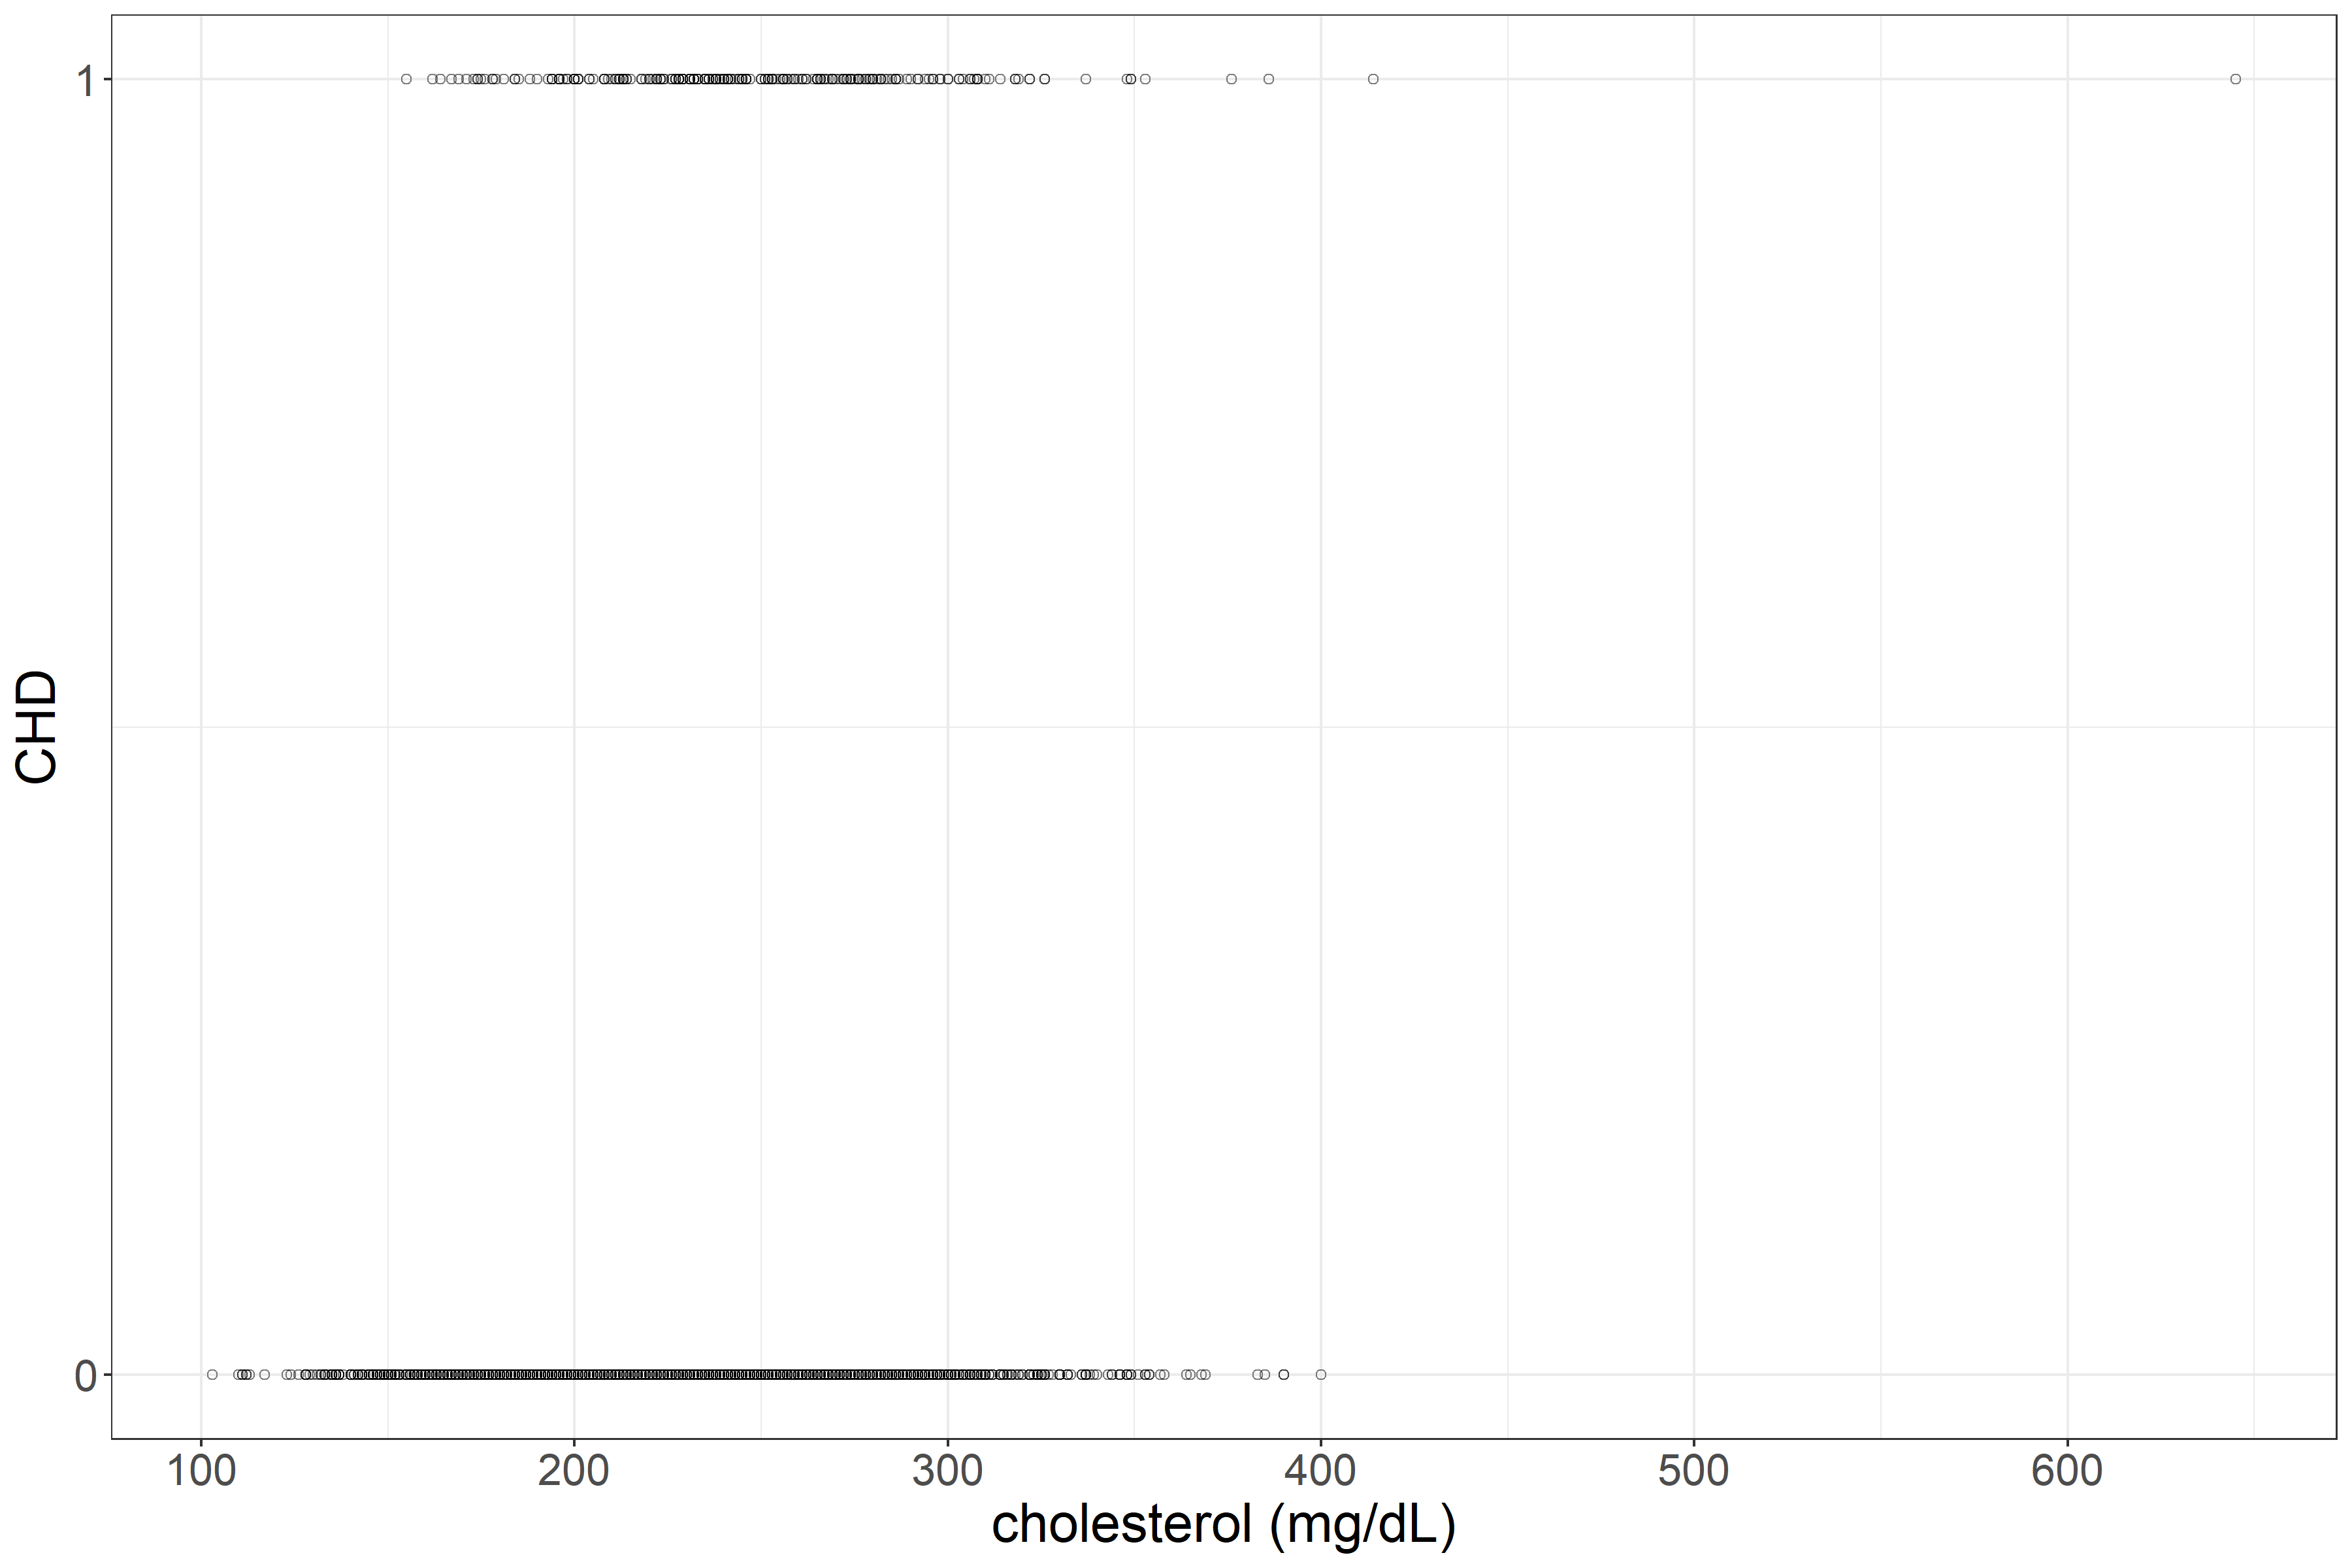
\includegraphics[width=0.7\textwidth]{./figs/scatter}
	\end{center}
\end{frame}

% graphical support: scatterplot
\begin{frame}{Linear regression with binary outcomes: Graphical support}
	We can plot the linear regression fit for this model.
	\begin{align*} 
		E[\texttt{chd}|\texttt{chol}] = \beta_0 + \beta_1 \texttt{chol}  
	\end{align*}
	
	\color{blue} Graphical support: \color{black} scatterplot with least squares line
	
	\begin{center}
		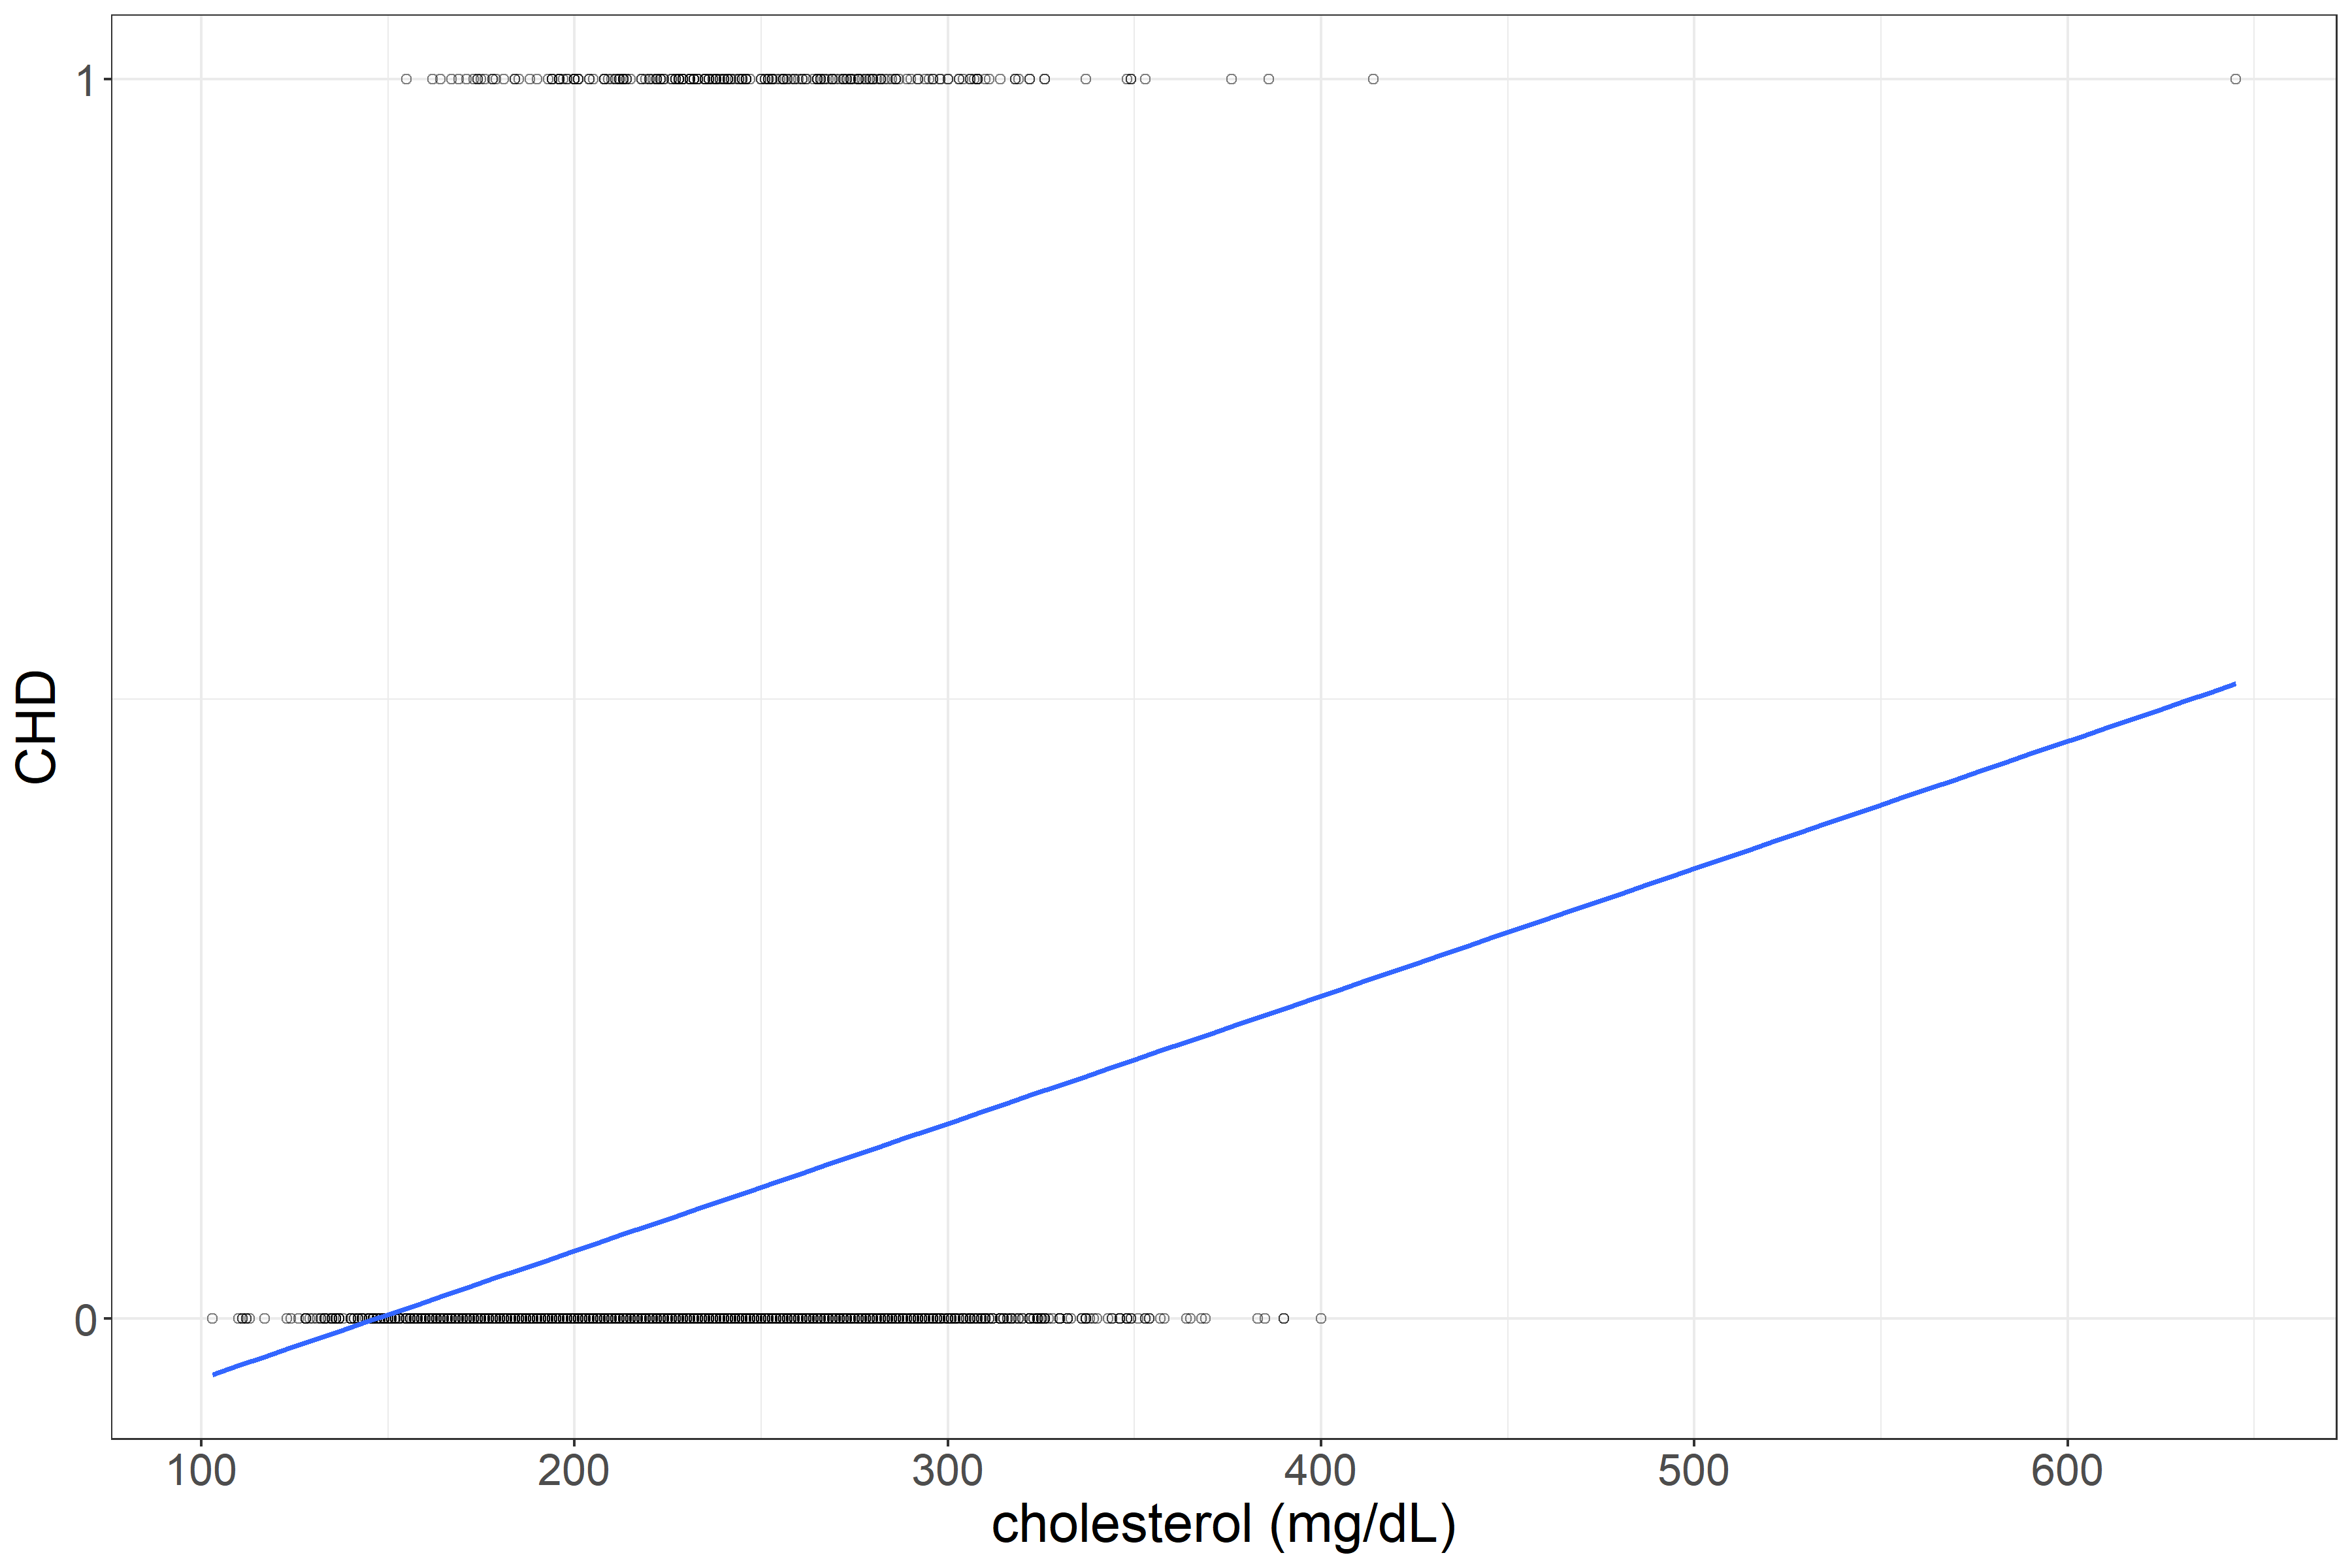
\includegraphics[width=0.7\textwidth]{./figs/scatter_lm}
	\end{center}
\end{frame}

\begin{frame}{Linear regression with binary outcomes: Graphical support}
	\vspace{-1cm}
	\begin{align*} 
		E[\texttt{chd}|\texttt{chol}] = \beta_0 + \beta_1 \texttt{chol}  
	\end{align*}
	What is the predicted probability of CHD for someone with cholesterol of 120 mg/dL?
	
	\begin{center}
		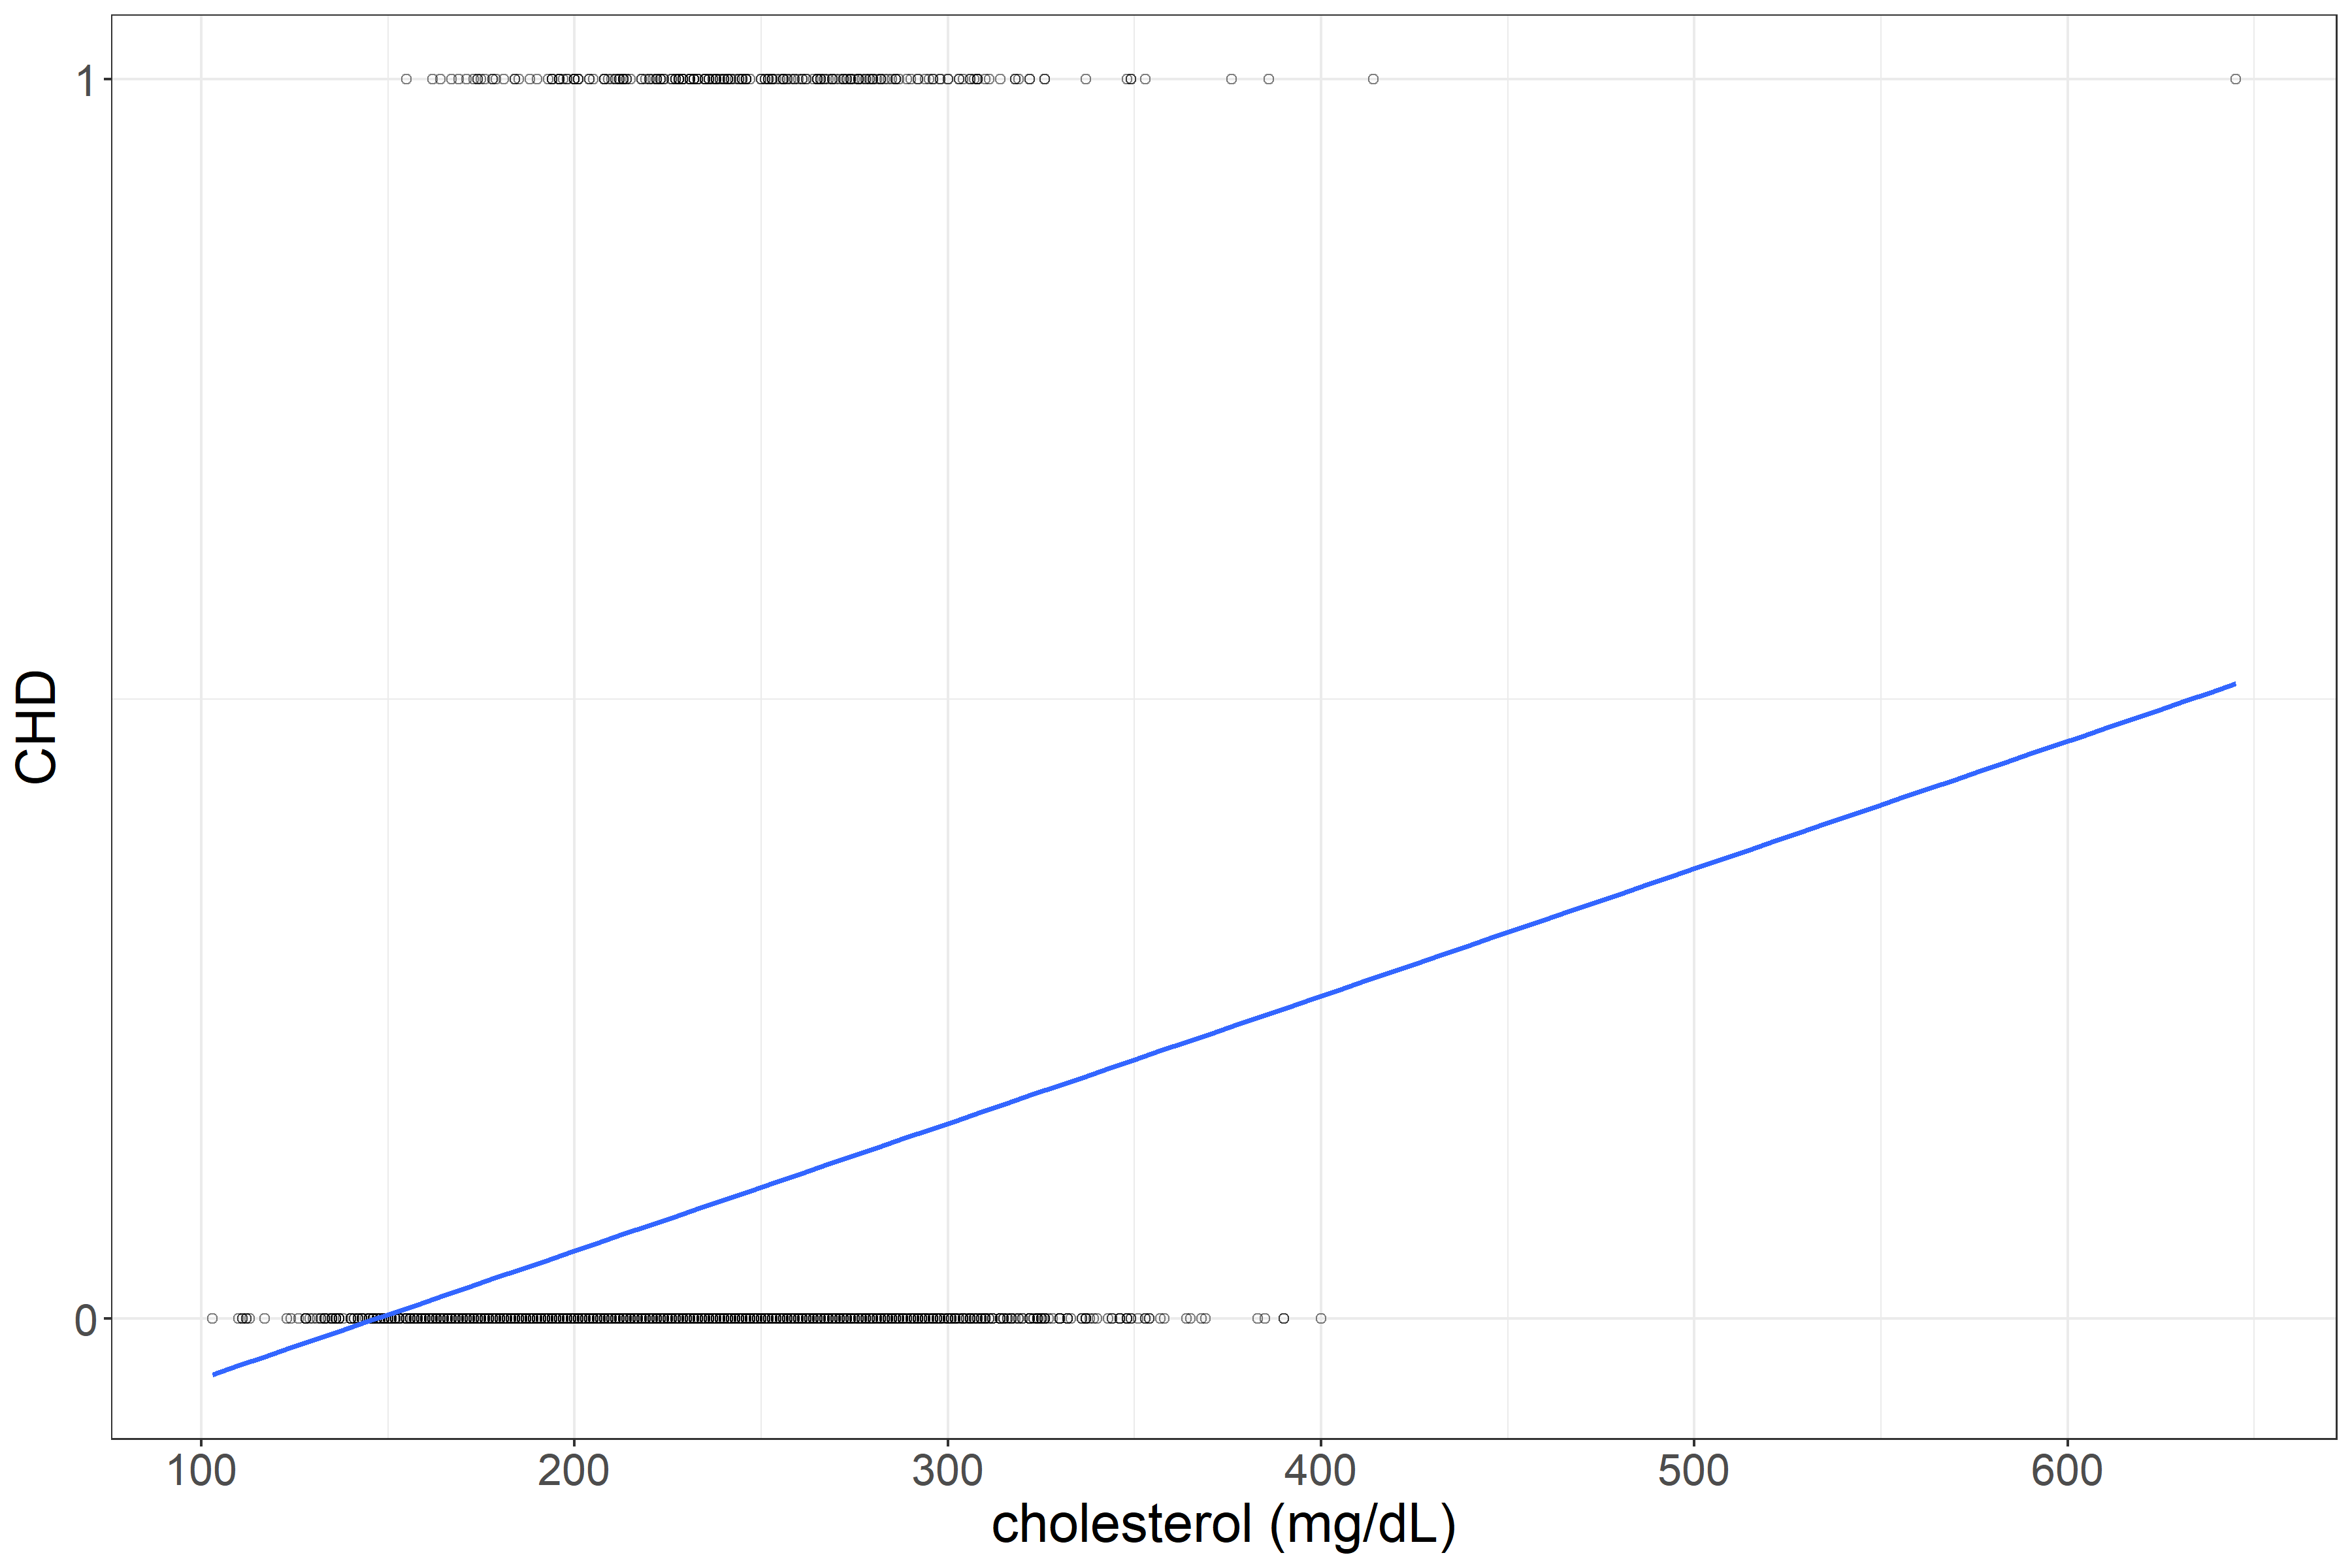
\includegraphics[width=0.7\textwidth]{./figs/scatter_lm}
	\end{center}
\end{frame}

\begin{frame}{Linear regression with binary outcomes: pros and cons}
	\begin{align*} 
		E[Y|X_1,\cdots,X_p] = \beta_0 + \beta_1 X_1 + \beta_2 X_2 + \cdots \beta_p X_p 
	\end{align*}
	
	Pros: 
	\begin{itemize}
		\item Coefficients and predictions are easy to interpret since they are on the probability scale
	\end{itemize}
	
	Cons: 
	\begin{itemize}
		\item Predicted/fitted values can be outside the (0,1) range (as we just saw in the cholesterol example)
		\item Our mean model might not be correct (particularly the linearity assumption)% is one of the assumptions for linear regression that actually is important
	\end{itemize}
	
	\textbf{What can we do instead?}
\end{frame}


%%% LOGISTIC REGRESSION %%%
\section{Logistic regression}
\begin{frame}
	\frametitle{SECTION 3: LOGISTIC REGRESSION}
	% Learning objectives
	By the end of this section, you should be able to:
	\begin{itemize}
		\item Interpret regression coefficients for simple and multiple logistic regression models
		\item Formulate a logistic regression model given a scientific or statistical question 
		\item Use \texttt{R} to fit a logistic regression model and extract relevant results
		\item Write a summary of results from a logistic regression analysis
		\item Describe the impact of including (or not including) a confounder or precision variable in logistic regression
		\item List at least one advantage and one disadvantage of using logistic regression with a binary outcome
	\end{itemize}
\end{frame}

\subsection{Simple logistic regression}
% motivating logistic regression
\begin{frame}
	\frametitle{CHD versus Type A behavior: odds}
	\vspace{-0.5cm}
	\begin{small} What if we wanted to quantify the association between CHD and Type A behavior via the \textit{odds ratio} rather than the \textit{risk difference}? \end{small} \pause

	\begin{enumerate}
			\item \textbf{Scientific Question:} is Type A behavior \textcolor{orange}{associated} with the risk of CHD? \pause
			\item \textbf{Statistical Question:} is the \textcolor{orange}{ratio of odds} of CHD between people with and without Type A behavior different from 1? \pause
			\begin{itemize}
					\item \textbf{Parameter:} odds ratio \pause
				\end{itemize}
			\item Take a \textbf{sample} from the population: cohort study of men in California aged 39-59 \pause
			\item Perform \textit{statistical inference}:
			\begin{itemize}
					\item Calculate a corresponding \textbf{statistic}: sample odds ratio
					\item Quantify uncertainty in your statistic
					\item Perform a hypothesis test \pause
				\end{itemize}
		\end{enumerate}
	
	\vspace{-0.2cm}
	We can use \textcolor{blue}{logistic} regression to answer this question!
\end{frame}

\begin{frame}{Thinking on the odds scale}
	As we've seen, the odds can take values from 0 to $\infty$. 
	\\ ~\
	
	Fitting a regression model on a variable with a restricted range can cause issues with values falling outside the possible range. We saw this a few slides ago with linear regression!
	\\ ~\
	
	Solution: Apply the $log$ function to the odds. 
	%%% INSERT FIGURE HERE
\end{frame}

\begin{frame}{Brief review of logarithms}
	\vspace{-0.6cm}
	In statistics, we generally deal with the natural logarithm, which has base $e$. You may have seen this written as \textcolor{blue}{$\ln$}, but we will use \textcolor{blue}{$\log$}. 
	\\ ~\
	
	The logarithm of $x$ is the number $b$ such that $e^b = x$, i.e. the power to which you raise $e$ to get $x$. 
	\\ ~\
	
	This might seem like an odd function to use, but logarithms take nonnegative numbers and map them to $(-\infty, \infty)$, which lets us not worry about restricted ranges. 
	
	\begin{center}
		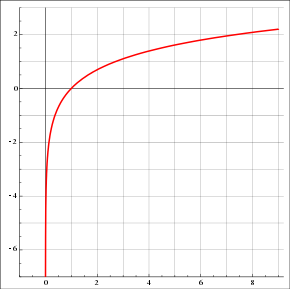
\includegraphics[width=0.4\textwidth]{./figs/log}
	\end{center}
\end{frame}

\begin{frame}{Brief review of logarithms}
	Two very useful properties of logarithms for you to know: 
	\begin{itemize}
		\item The logarithm is the inverse of the exponential function:
		\begin{align*}
			e^{\log(x)} = x \tab \text{and} \tab \log(e^x) = x
		\end{align*}
	
		\item The logarithm of a quotient is the difference of the logarithms:
		\begin{align*}
			\log(x/y) = \log(x) - \log(y)
		\end{align*}
	\end{itemize}
\end{frame}

% simple logistic regression recall
\begin{frame}{Simple logistic regression: interpretation}
	\textbf{Discuss with your neighbor:}
	\\ ~\
	
	Suppose we fit the simple logistic regression model $$\log\left(\text{Odds}[Y =1 \mid X]\right) = \beta_0 + \beta_1 X,$$ where our outcome $Y$ is binary. What is the interpretation of the following quantities?
	\begin{enumerate}
		\item $\beta_0$
		\item $\beta_1$
		\item $\exp(\beta_0)$
		\item $\exp(\beta_1)$
	\end{enumerate} 
\end{frame}

% simple logistic regression recall
\begin{frame}{Simple logistic regression: interpretation}
	Suppose we fit the simple logistic regression model $$\log\left(\text{Odds}[Y =1 \mid X]\right) = \beta_0 + \beta_1 X,$$ where our outcome $Y$ is binary. What is the interpretation of the following quantities?
	\begin{enumerate}
		\item $\beta_0$: log odds of $Y = 1$ when $X = 0$
		$$\log\left(\text{Odds}[Y =1 \mid X = 0]\right) = \beta_0 + \beta_1\times 0$$
	\end{enumerate} 
\end{frame}

% simple logistic regression recall
\begin{frame}{Simple logistic regression: interpretation}
	Suppose we fit the simple logistic regression model $$\log\left(\text{Odds}[Y =1 \mid X]\right) = \beta_0 + \beta_1 X,$$ where our outcome $Y$ is binary. What is the interpretation of the following quantities?
	\begin{enumerate}
		\item[2.] $\beta_1$: difference in log odds of $Y = 1$ comparing $X = 1$ and $X =0$ groups
	\end{enumerate} 
	\begin{align*}
	&\log\left(\text{Odds}[Y =1 \mid X = x]\right) = \beta_0 + \beta_1x\\
	&\log\left(\text{Odds}[Y =1 \mid X = x + 1]\right) = \beta_0 + \beta_1(x + 1)\\
	&\Rightarrow \log\left(\text{Odds}[Y =1 \mid X = x + 1]\right) - \log\left(\text{Odds}[Y =1 \mid X = x ]\right) = \beta_1
\end{align*}
\end{frame}

% simple logistic regression recall
\begin{frame}{Simple logistic regression: interpretation}
	Suppose we fit the simple logistic regression model $$\log\left(\text{Odds}[Y =1 \mid X]\right) = \beta_0 + \beta_1 X,$$ where our outcome $Y$ is binary. What is the interpretation of the following quantities?
	\begin{enumerate}
		\item[3.] $\exp(\beta_0)$: odds of $Y = 1$ when $X = 0$
	\end{enumerate} 
	\begin{align*}
	&\log\left(\text{Odds}[Y =1 \mid X = 0]\right) = \beta_0\\
	&\Rightarrow \exp(\log(\text{Odds}[Y =1 \mid X = 0])) = \exp(\beta_0)\\
	&\Rightarrow \text{Odds}[Y =1 \mid X = 0] = \exp(\beta_0)
	\end{align*}
\end{frame}

% simple logistic regression recall
\begin{frame}{Simple logistic regression: interpretation}
	Suppose we fit the simple logistic regression model $$\log\left(\text{Odds}[Y =1 \mid X]\right) = \beta_0 + \beta_1 X,$$ where our outcome $Y$ is binary. What is the interpretation of the following quantities?
	\begin{enumerate}
		\item[4.] $\exp(\beta_1)$: ratio of odds of $Y = 1$ comparing $X = 1$ and $X = 0$ groups
	\end{enumerate} 
\begin{footnotesize}
	\begin{align*}
		&\log\left(\text{Odds}[Y =1 \mid X = x + 1]\right) - \log\left(\text{Odds}[Y =1 \mid X = x ]\right) = \beta_1\\
		&\Rightarrow \exp(\log\left(\text{Odds}[Y =1 \mid X = x + 1]\right) - \log\left(\text{Odds}[Y =1 \mid X = x ]\right)) = \exp(\beta_1)\\
		&\Rightarrow \exp\biggr(\log\biggr(\frac{\text{Odds}[Y =1 \mid X = x + 1]}{\text{Odds}[Y =1 \mid X = x ]}\biggr)\biggr) = \exp(\beta_1)\\
		&\Rightarrow \frac{\text{Odds}[Y =1 \mid X = x + 1]}{\text{Odds}[Y =1 \mid X = x ]} = \exp(\beta_1)
	\end{align*}
\end{footnotesize}
\end{frame}

% simple logistic regression recall
\begin{frame}{Simple logistic regression: interpretation}
	Suppose we fit the simple logistic regression model $$\log\left(\text{Odds}[Y =1 \mid X]\right) = \beta_0 + \beta_1 X,$$ where our outcome $Y$ is binary. What is the interpretation of the following quantities?
	\begin{enumerate}
		\item $\beta_0$: log odds of $Y = 1$ when $X = 0$ \pause
		\item $\beta_1$: difference in log odds of $Y = 1$ comparing $X = 1$ and $X =0$ groups \pause
		\item $\exp(\beta_0)$: odds of $Y = 1$ when $X = 0$ \pause
		\item $\exp(\beta_1)$: ratio of odds of $Y = 1$ comparing $X = 1$ and $X = 0$ groups (\textcolor{blue}{in other words, the odds ratio!})
	\end{enumerate} 
\end{frame}

\subsection{Multiple logistic regression}
% interpretation: multiple/general, do the math
%%% beta 0
\begin{frame}
	\frametitle{Multiple logistic regression}
	\vspace{-1.5cm}
	$$\log\left(\text{Odds}[Y =1 |X_1,\cdots,X_p]\right) = \beta_0 + \beta_1 X_1 + \beta_2X_2 + \cdots \beta_p X_p$$
	
	\color{blue} Interpretation: \color{black}
	% beta0
	\begin{itemize}  \color{red}
		\item $\beta_0$: \pause log odds (of $Y=1$) when $X_1 = 0, \cdots, X_p = 0$ \pause
	\end{itemize}
	\vspace{-0.3cm}
	\begin{footnotesize}
		\begin{align*}
			\log\left(\text{Odds}[Y =1 |X_1=0,\cdots,X_p=0]\right) & = \beta_0 + \beta_1 (0) + \beta_2(0) + \cdots \beta_p (0) \\
			& = \beta_0 
		\end{align*} \pause
	\end{footnotesize}
	
	\vspace{-0.6cm}
	%exp(beta0)
	\begin{itemize}   \color{red}
		\item $e^{\beta_0}$: \pause odds (of $Y=1$) when $X_1 = 0, \cdots, X_p = 0$ \pause
	\end{itemize}
	\vspace{-0.3cm}
	\begin{footnotesize}
		\begin{align*}
			e^{\beta_0} & = e^{\log\left(\text{Odds}[Y =1 |X_1=0,\cdots,X_p=0]\right)} \\
			& = \text{Odds}[Y =1 |X_1=0,\cdots,X_p=0]
		\end{align*}
	\end{footnotesize}
\end{frame}

% interpretation: multiple/general, do the math
%%% beta 0
\begin{frame}
	\frametitle{Multiple logistic regression}
	\vspace{-1.5cm}
	$$\log\left(\text{Odds}[Y =1 |X_1,\cdots,X_p]\right) = \beta_0 + \beta_1 X_1 + \beta_2X_2 + \cdots \beta_p X_p$$
	
	\color{blue} Interpretation: \color{black}
	%exp(beta0)
	\begin{itemize}   \color{red}
		\item $\beta_1$: \pause difference in log odds (of $Y=1$) comparing groups that differ by 1 unit in $X_1$ but are the same with respect to $X_2, \dots, X_p$ \pause
	\end{itemize}
	\vspace{-0.3cm}
	\begin{footnotesize}
		\begin{align*}
			&\log\left(\text{Odds}[Y =1 |X_1=x_1+1,X_2 = x_2\cdots,X_p=x_p]\right) \\
			&\tab - \log\left(\text{Odds}[Y =1 |X_1=x_1,X_2 = x_2\cdots,X_p=x_p]\right) \\
			& = (\beta_0 + \beta_1(x_1+1) + \beta_2x_2 + \cdots \beta_px_p) - (\beta_0 + \beta_1x_1 + \beta_2x_2 + \cdots \beta_px_p) \\
			& = \beta_1
		\end{align*}
	\end{footnotesize}\pause
	\vspace{-0.3cm}
	\begin{itemize}\color{red}
			\item $e^\beta_1$: \pause odds ratio (of $Y = 1$) comparing groups that differ by 1 unit in $X_1$ but are the same with respect to $X_2,\dots, X_p$ 
	\end{itemize}\pause
\vspace{-0.3cm}
\begin{footnotesize}
\begin{align*}
	e^{\beta_1} &=\exp\biggr(\log\left(\text{Odds}[Y =1 |X_1=x_1+1,X_2 = x_2\cdots,X_p=x_p]\right) \\
	&\tab - \log\left(\text{Odds}[Y =1 |X_1=x_1,X_2 = x_2\cdots,X_p=x_p]\right)\biggr) \\
	&= \exp\biggr(\log\biggr(\frac{\text{Odds}[Y =1 |X_1=x_1+1,X_2 = x_2\cdots,X_p=x_p]}{\text{Odds}[Y =1 |X_1=x_1,X_2 = x_2\cdots,X_p=x_p]}\biggr)\biggr)\\
	& = \frac{\text{Odds}[Y =1 |X_1=x_1+1,X_2 = x_2\cdots,X_p=x_p]}{\text{Odds}[Y =1 |X_1=x_1,X_2 = x_2\cdots,X_p=x_p]}
\end{align*}
\end{footnotesize}
\end{frame}

\begin{frame}{Example: CHD and \textit{arcus senilis}}
	Let's return to our study of CHD and \textit{arcus senilis}.
	\\ ~\
	
	The \texttt{wcgs} has some other available information on the subjects in the study (this is not a complete list):
	\begin{itemize}
		\item Patient ID
		\item Age (years)
		\item Height (inches)
		\item Weight (lbs)
		\item Systolic blood pressure (mmHg)
		\item Diastolic blood pressure (mmHg)
		\item Cholesterol (mg/dL)
	\end{itemize}  

	\textbf{We are interested in assessing the potential association between \textit{arcus senilis} and risk of CHD.} 
\end{frame}

\begin{frame}{Logistic regression: formulating a statistical question}
	\begin{enumerate}
		\item \textbf{Scientific Question:} \pause Is \textit{arcus senilis} associated with risk of CHD? \pause
		\item \textbf{Statistical Question:} \pause 
		\begin{itemize}
			\item How is our outcome quantified? \begin{tiny}The study is already completed -- we don't really have any control over this!\end{tiny}\pause
			\item[] \textcolor{blue}{Binary: cardiovascular event = 1, no event = 0}\pause
			\item How will we quantify association? \pause
			\item[] \textcolor{blue}{Ratio of odds of CHD comparing groups with and without \textit{arcus senilis}}\pause
			\item Are there other variables we should adjust for?\pause
			\item[] \textcolor{blue}{Draw the causal diagram!}\pause
		\end{itemize}
	\end{enumerate}\pause
\vspace{1cm}
Is the odds ratio of CHD different from 1 comparing subjects with and without \textit{arcus senilis} of the same age, weight, systolic blood pressure, diastolic blood pressure, and cholesterol? 
\end{frame}

\begin{frame}{Logistic regression: writing the regression model}
	Is the odds ratio of CHD different from 1 comparing subjects with and without \textit{arcus senilis} of the same age, weight, systolic blood pressure, diastolic blood pressure, and cholesterol? 
	\\ ~\ 
	
	\textbf{Regression Model:} \pause
	\begin{align*}
		\log(&\text{Odds}[\texttt{chd} \mid \texttt{arcus}, \texttt{age}, \texttt{weight}, \texttt{sbp}, \texttt{dbp}, \texttt{chol}]) \\
		&= \beta_0 + \beta_1\texttt{arcus} + \beta_2\texttt{age} + \beta_3\texttt{weight} \\
		&\tab + \beta_4\texttt{sbp} + \beta_5\texttt{dbp} + \beta_6\texttt{chol}
	\end{align*}
\end{frame}

\begin{frame}{
\includegraphics[scale=0.01]{./figs/chilipepper} Terminology}
	You will often seen logistic regression framed a bit differently than what we've seen so far. \pause
	\\ ~\ 
	
	You may see
	\begin{align*}
		\text{logit}(P[Y = 1 \mid X]) = \beta_0 + \beta_1 X
	\end{align*}
where the logit function is defined as \pause
\begin{align*}
	\text{logit}(p) = \log\Big(\underbrace{\frac{p}{1-p}}_{\text{odds}}\Big)
\end{align*}
\pause
Formally, the logit function is called a \textcolor{blue}{link} function, since it links our mean $E[Y \mid X] = P[Y = 1 \mid X]$ to our model $\beta_0 + \beta_1 X$. 
\end{frame}

\begin{frame}{Logistic regression: fitting the model in \texttt{R}}
	The \texttt{lm} function won't do it for us anymore. Instead we use the \texttt{glm} function. 
	\\ ~\ 
	
	GLM stands for ``generalized linear model" and represents a whole class of regression methods (more on that later!). For now, all you need to know is that \texttt{glm} syntax is a lot like \texttt{lm} syntax, but we must also specify $\texttt{family = binomial()}$. 
\end{frame}

\begin{frame}{Logistic regression: \texttt{R} output}
	\vspace{-1cm}
		\begin{center}
		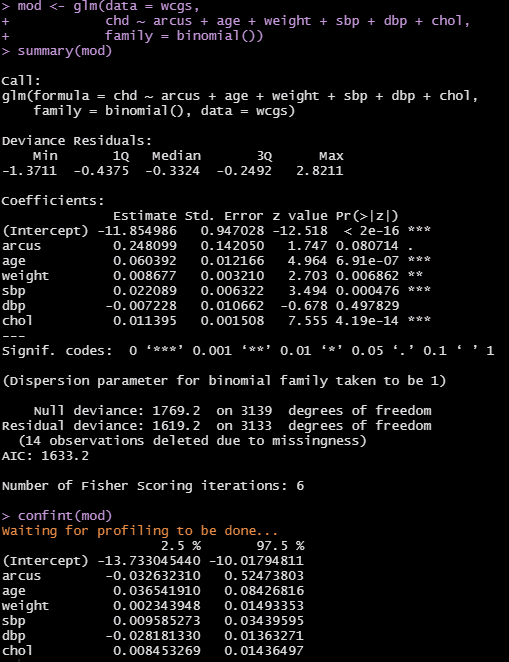
\includegraphics[width=0.6\textwidth]{./figs/multiple_logistic_regression_arcus}
	\end{center}
\end{frame}

\begin{frame}{Logistic regression: transforming \texttt{R} output}
	\vspace{-0.7cm}
	As you could infer by the fact that some estimates were negative, \texttt{R} has given us the raw regression coefficient estimates and intervals. But as we've seen, the exponentiated versions are much more interpretable!
			\begin{center}
		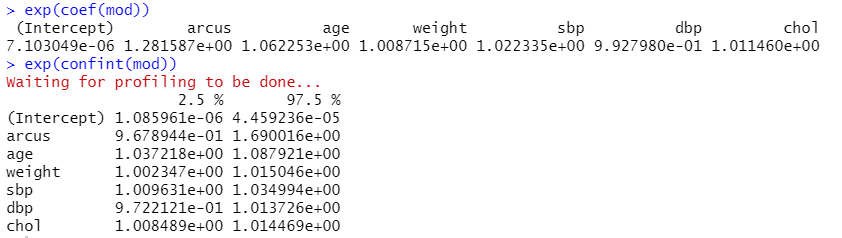
\includegraphics[width=\textwidth]{./figs/multiple_logistic_regression_arcus_exp}
	\end{center}
	We can use \texttt{coef} to pull out coefficients, and then exponentiate (same for \texttt{confint}).
	\\ ~\
	
	Note: The p-values for the hypothesis tests can be used directly since a test of $H_0: \beta_1 = 0$ is the same as a test of $H_0: \exp(\beta_1) = 1$. More on this in a few slides!
\end{frame}

\begin{frame}{Logistic regression: reporting results}
	\begin{enumerate}
		\item[4.] Perform \textit{statistical inference}:
		\begin{itemize}
			\item Calculate a test statistic: odds ratio of 1.28
			\item Quantify uncertainty: 95\% CI of (0.97, 1.69)
			\item Perform hypothesis test: $p = 0.08$
		\end{itemize}
		\item[5.] Add a conclusion
	\end{enumerate}
	Based on logistic regression, we estimate that the odds of CHD are 1.28 times as high in subjects with \textit{arcus senilis} versus those without, comparing subjects of the same age, weight, systolic blood pressure, diastolic blood pressure, and cholesterol. The data would be consistent with a true odds ratio between 0.97 and 1.69. Based on a test of the null hypothesis of an odds ratio of 1, there is not sufficient evidence of an association between \textit{arcus senilis} and CHD (p = 0.08), after adjusting for age, weight, blood pressure, and cholesterol. 
\end{frame}

\begin{frame}{A note on confidence intervals and p-values}
	\vspace{-0.7cm}
	Suppose I fit the simple model $\log(\text{Odds}(\texttt{chd} \mid \texttt{arcus})) = \beta_0 + \beta_1 \texttt{arcus}$ and get the following \texttt{R} output, with exponentiated point estimates and intervals: 
	
	\begin{center}
	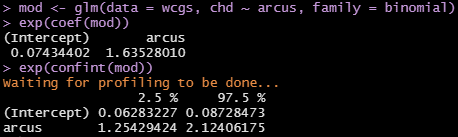
\includegraphics[width=0.5\textwidth]{./figs/asymmetric_CI}
	\end{center}
	For the \texttt{arcus} predictor, we have a point estimate of 1.64 with 95\% CI (1.25, 2.12). It's a bit subtle, but this CI isn't actually symmetric about our point estimate!
		\begin{center}
		
\includegraphics[width=0.5\textwidth]{./figs/asymmetric_CI_pic}
	\end{center}
\end{frame}

\begin{frame}{A note on confidence intervals and p-values}
	What's going on here? 
	\\ ~\
	
	\texttt{glm} is working on the log-odds scale:
	\begin{align*}
		&\text{Confidence interval: }(\hat{\beta} - 1.96 \times \hat{\text{SE}}, \hat{\beta} + 1.96 \times \hat{\text{SE}})\\
		&\text{Hypothesis test: }H_0: \beta = 0 \tab H_1: \beta \neq 0
	\end{align*}
	When you exponentiate to the odds scale, the interval is longer symmetric and the hypotheses are different:
	\begin{align*}
		&\text{Confidence interval: }(e^{\hat{\beta} - 1.96 \times \hat{\text{SE}}}, e^{\hat{\beta} + 1.96 \times \hat{\text{SE}}})\\
		&\text{Hypothesis test: }H_0: \exp(\beta) = 1 \tab H_1: \exp(\beta) \neq 1
	\end{align*} 
	The p-values are unaffected (if the log-odds scale CI doesn't overlap 0, then the odds scale CI won't overlap 1)
\end{frame}


\subsection{Prediction}
\begin{frame}{Logistic regression: Prediction}
	We can also use logistic regression for prediction, though it takes a bit more work to get results on the scale we want. 
	\\ ~\
	
	Let's start with the a single quantitative predictor, cholesterol:
	\begin{align*}
		\log(\text{Odds}(\texttt{chd} \mid \texttt{chol})) = \beta_0 + \beta_1 \texttt{chol}
	\end{align*}
	\begin{center}
	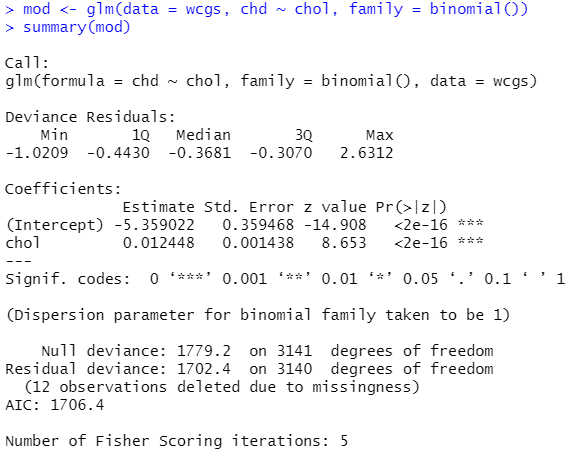
\includegraphics[width=0.5\textwidth]{./figs/simple_logistic_regression_chol}
\end{center}
\end{frame}

\begin{frame}{Logistic regression: Prediction}
	\vspace{-1cm}
		\begin{align*}
		\log(\text{Odds}(\texttt{chd} \mid \texttt{chol})) = \beta_0 + \beta_1 \texttt{chol}
	\end{align*}
	Let's predict for a person with a cholesterol of 220 mg/dL:
	\begin{enumerate}
		\item Get estimates for each regression coefficient: 
		\item[] $\hat{\beta}_0 = -5.359, \hat{\beta}_1 = 0.0124$
		\item Plug in estimates and predictor values:
		\begin{enumerate}
			\item[a.] $\widehat{\log(\text{Odds})} = -5.359 + (0.0124\times220$) = -2.62
			\item[b.] $\widehat{\text{Odds}} = e^{-2.62} = 0.0728$
			\item[] \textcolor{blue}{(using that $e^{\log x} = x$)}
			\item[c.] $\widehat{\text{Prob}} = \frac{0.0659}{1 + 0.0659} = 0.068$
			\item[] \textcolor{blue}{(using that Odds = $\frac{\text{Prob}}{1-\text{Prob}}$ and so Prob = $\frac{\text{Odds}}{1  +\text{Odds}}$)}
		\end{enumerate}
	\end{enumerate}
	There's a common shortcut to get from \textcolor{blue}{a.} to our final answer. 
	\begin{align*}
		\text{expit}(x) = \frac{e^x}{1 + e^x} \Rightarrow \text{expit}(-2.719) = 0.068
	\end{align*}
\end{frame}

\begin{frame}{Logistic regression: Prediction}
	Of course, \texttt{R} will do all the work for us: 
	\begin{center}
		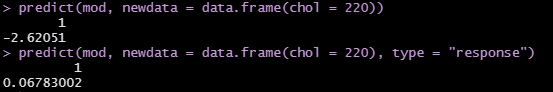
\includegraphics[width=0.8\textwidth]{./figs/simple_logistic_regression_chol_prediction}
	\end{center}
	We need to use \texttt{type = "response"} to predict on the probability scale
\end{frame}

\begin{frame}{Logistic regression: Prediction}
	Unlike linear regression (blue), logistic regression (red) keeps all fitted and predicted values in [0,1]
		\begin{center}
		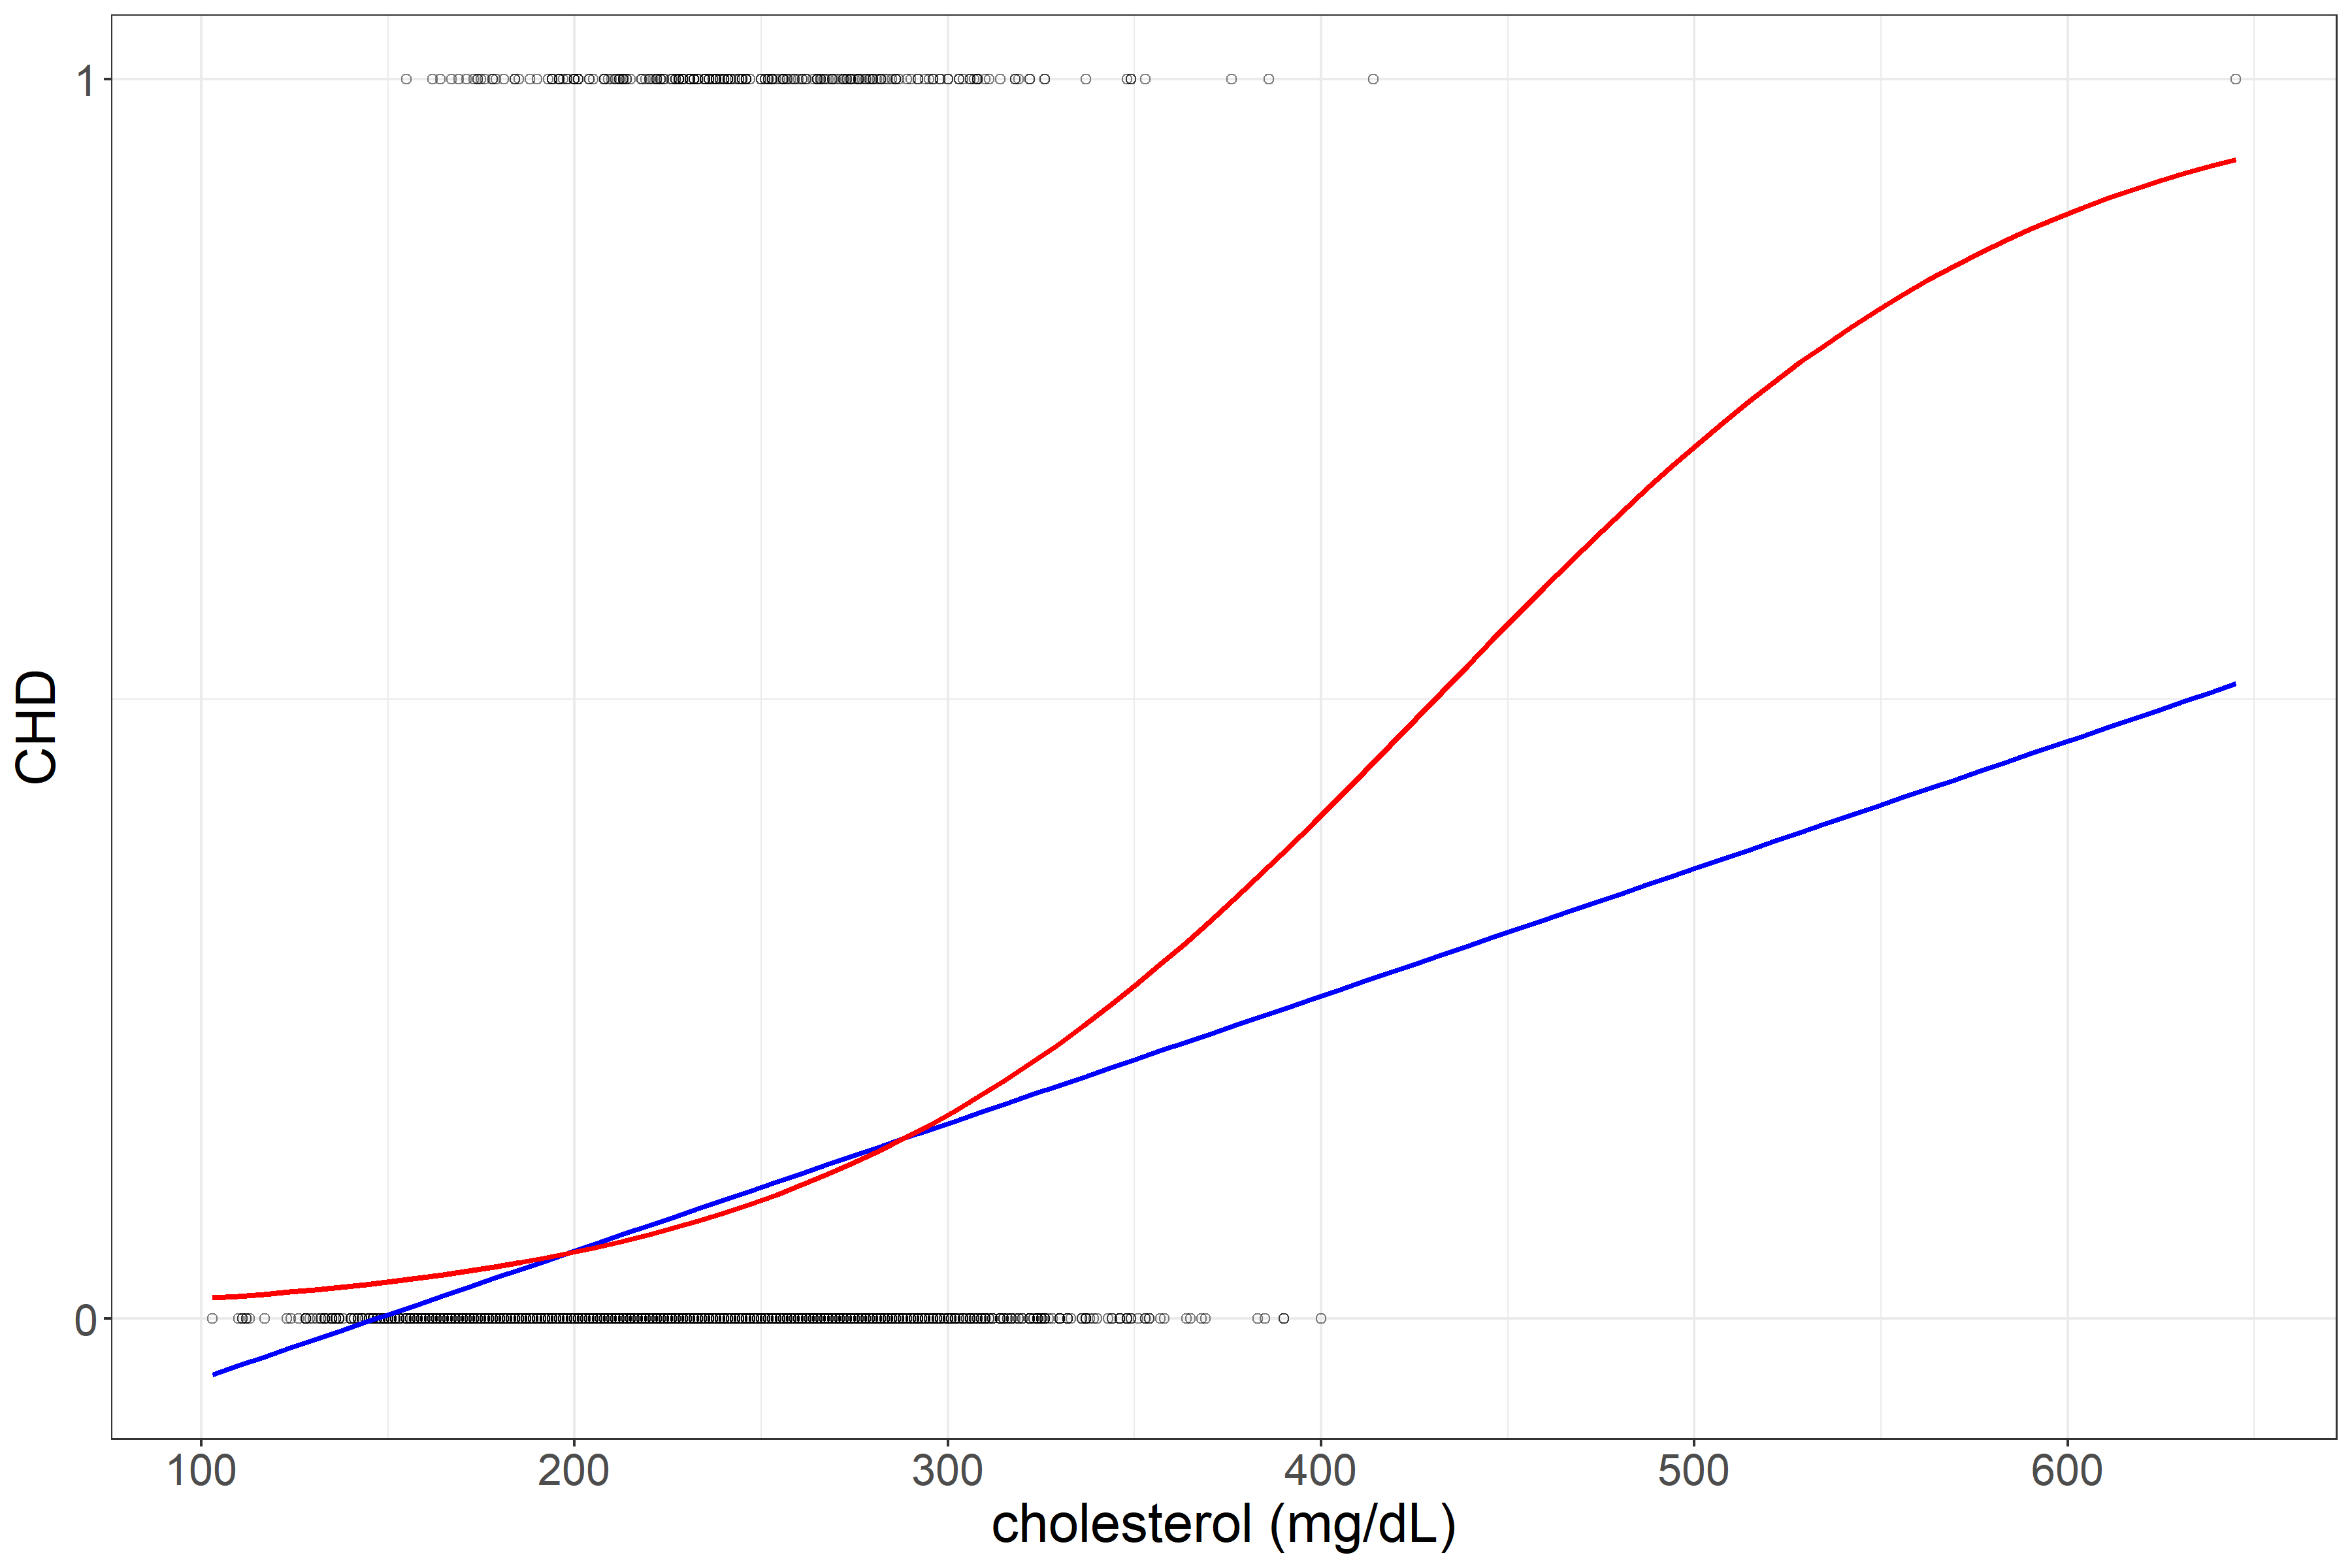
\includegraphics[width=0.8\textwidth]{./figs/scatter_glm}
	\end{center}
\end{frame}

\begin{frame}{Logistic regression: pros and cons}
	\begin{align*}
		\log(\text{Odds}[Y = 1 \mid X_1,\dots, X_p]) = \beta_0 + \beta_1X_1 + \beta_2X_2 + \cdots + \beta_pX_p
	\end{align*}
	Pros:
	\begin{itemize}
		\item Predicted/fitted values stay inside [0,1] range
		\item Allows analysis of case-control studies (see next section!)
		\item 
\includegraphics[scale=0.01]{./figs/chilipepper} Numerically stable: We don't get into the details here, but some other options for binary outcome regression have major computational issues!
	\end{itemize}
	Cons:
	\begin{itemize}
		\item Harder to interpret (odds and odds ratios)
	\end{itemize}
\end{frame}

\section{Case-control studies}
\begin{frame}
	\frametitle{SECTION 4: CASE-CONTROL STUDIES}
	% Learning objectives
	By the end of this section, you should be able to:
	\begin{itemize}
		\item Describe why logistic regression is useful for the analysis of case-control data
		\item Explain how and why logistic regression interpretation changes when we analyze case-control data
	\end{itemize}
\end{frame}

\begin{frame}{Recall: case-control study}
	Description:
	\begin{itemize}
		\item \textit{Sample individuals based on the outcome} (some with, some without) and look back in time for exposure. 
	\end{itemize}\pause
	Pros:\pause
	\begin{itemize}
		\item Efficient for rare outcomes\pause
		\item Cheaper and faster than cohort studies\pause
		\item Can study multiple exposures\pause
	\end{itemize}
	
	Cons:\pause
	\begin{itemize}
		\item In some scenarios, may not know time sequence of disease and exposure\pause
		\item \textcolor{red}{Cannot use to estimate relative risk or outcome prevalence}\pause
		\item Potential confounding (cannot make conclusions about causality)\pause
	\end{itemize}
\end{frame}

\begin{frame}{Why can't we estimate RR or prevalence from case-control?}
	\textbf{In case-control studies, we cannot estimate relative risk or disease prevalence.}
	\\ ~\
	
	Why not? 
	\begin{itemize}
		\item This is a biased sampling scheme
		\item We do \textbf{not} have a representative sample of the population. We purposely sample more individuals who have the outcome ($Y = 1$) than we would 
		get from a simple random sample
			\begin{itemize}
				\item This is by design, and precisely why case-control studies are more efficient for rare outcomes!
			\end{itemize}
		\item Within categories $Y = 1$ (cases) and $Y = 0$ (controls), the samples should be representative but the overall sample is not
	\end{itemize} 
\end{frame}

\begin{frame}{Case-control sampling: Example}
	\vspace{-0.3cm}
	To illustrate this, consider the following \textcolor{blue}{population} of 1 million individuals:
	\begin{center}
		\begin{table}
			\begin{tabular}{|c|cc|c|}
				\hline 
				& Lung Cancer & No Lung Cancer &  \\ 
				& (Case) & (Control) & Total  \\
				\hline 
				Smoke & 900 & 4,100  & 5,000 \\ 
				No Smoke & 100 & 994,900 & 995,000  \\ 
				\hline 
				Total & 1000 & 999,000 & 1,000,000 \\ 
				\hline 
			\end{tabular}
		\end{table}
	\end{center}\pause
	We are doing a case-control study on lung cancer and smoking. We have the resources to sample 400 individuals. We randomly pick 200 people with lung cancer and 200 without. Here's our \textcolor{blue}{sample}:
		\begin{center}
		\begin{table}
			\begin{tabular}{|c|cc|c|}
				\hline 
				& Lung Cancer & No Lung Cancer &  \\ 
				& (Case) & (Control) & Total  \\
				\hline 
				Smoke & 184 & 2  & 186 \\ 
				No Smoke & 16 & 198 & 214  \\ 
				\hline 
				Total & 200 & 200 & 400 \\ 
				\hline 
			\end{tabular}
		\end{table}
	\end{center}
\end{frame}

\begin{frame}{Case-control sampling: Example}
	\vspace{-0.3cm}
	\textcolor{blue}{Population:}
	\begin{center}
	\begin{table}
		\begin{tabular}{|c|cc|c|}
			\hline 
			& Lung Cancer & No Lung Cancer &  \\ 
			& (Case) & (Control) & Total  \\
			\hline 
			Smoke & 900 & 4,100  & 5,000 \\ 
			No Smoke & 100 & 994,900 & 995,000  \\ 
			\hline 
			Total & 1000 & 999,000 & 1,000,000 \\ 
			\hline 
		\end{tabular}
	\end{table}
\end{center}\pause
The prevalence of lung cancer in the \textcolor{blue}{population} is
\begin{align*}
	P^{\text{pop}}(\text{cancer}) = \frac{1,000}{1,000,000} = 0.001
\end{align*}\pause
The prevalence of lung cancer among smokers and nonsmokers is
\begin{align*}
	&P^{\text{pop}}(\text{cancer} \mid \text{smoke}) = \frac{900}{5,000} = 0.18\\
	&P^{\text{pop}}(\text{cancer} \mid \text{no smoke}) = \frac{100}{995,000} = 0.0001
\end{align*}
\end{frame}

\begin{frame}{Case-control sampling: Example}
	\vspace{-0.3cm}
	\textcolor{blue}{Sample:}
		\begin{center}
	\begin{table}
		\begin{tabular}{|c|cc|c|}
			\hline 
			& Lung Cancer & No Lung Cancer &  \\ 
			& (Case) & (Control) & Total  \\
			\hline 
			Smoke & 184 & 2  & 186 \\ 
			No Smoke & 16 & 198 & 214  \\ 
			\hline 
			Total & 200 & 200 & 400 \\ 
			\hline 
		\end{tabular}
	\end{table}
\end{center}\pause
	The prevalence of lung cancer in the \textcolor{blue}{sample} is
	\begin{align*}
		P^{\text{samp}}(\text{cancer}) = \frac{200}{400} = 0.5 \tab \text{\textcolor{red}{(We chose this by design!)}}
	\end{align*}\pause
	The prevalence of lung cancer among smokers and nonsmokers is
	\begin{align*}
		&P^{\text{samp}}(\text{cancer} \mid \text{smoke}) = \frac{184}{186} = 0.989\\
		&P^{\text{samp}}(\text{cancer} \mid \text{no smoke}) = \frac{16}{214} = 0.075
	\end{align*}
\end{frame}

\begin{frame}{Case-control sampling: Example}
	\vspace{-1cm}
	\begin{align*}
		P^{\text{pop}}(\text{cancer}) = 0.001 \tab \text{vs.} \tab P^{\text{samp}}(\text{cancer}) = 0.5
	\end{align*}
	Clearly, our sample estimate of the prevalence of lung cancer is not even close to the true prevalence -- we chose half our sample to be cases, so the 0.5 was completely determined by us.
	\\ ~\
	
	Similarly, our prevalence estimates separated by exposure are way off:
	\begin{small} 
	\begin{align*}
		&P^{\text{pop}}(\text{cancer} \mid \text{smoke}) = 0.18 \hspace{0.5cm} \text{vs.} \hspace{0.5cm} P^{\text{samp}}(\text{cancer}\mid \text{smoke}) = 0.989\\
		&P^{\text{pop}}(\text{cancer}\mid \text{no smoke}) = 0.0001 \hspace{0.2cm} \text{vs.} \hspace{0.2cm} P^{\text{samp}}(\text{cancer}\mid \text{no smoke}) = 0.075
	\end{align*}
	\end{small}
	Because we \textcolor{blue}{oversampled} cases, both exposed and unexposed subjects appear to be at much higher risk of cancer than they actually are. 
\end{frame}

\begin{frame}{Case-control sampling: Example}
	\vspace{-1cm}
	What about the prevalence of smoking among those with and without lung cancer? \textcolor{red}{Because we randomly sampled within cases and within controls, we can estimate these!}
	\\ ~\
	
	\textbf{Exercise:} In both the population and the sample, calculate the prevalence of smoking among cases and controls.
	\\ ~\
	\vspace{-0.2cm}
	\textcolor{blue}{Population:} 
		\begin{center}
		\begin{table}
			\begin{tabular}{|c|cc|c|}
				\hline 
				& Lung Cancer & No Lung Cancer &  \\ 
				& (Case) & (Control) & Total  \\
				\hline 
				Smoke & 900 & 4,100  & 5,000 \\ 
				No Smoke & 100 & 994,900 & 995,000  \\ 
				\hline 
				Total & 1000 & 999,000 & 1,000,000 \\ 
				\hline 
			\end{tabular}
		\end{table}
	\end{center}
 \textcolor{blue}{Sample}:
	\begin{center}
		\begin{table}
			\begin{tabular}{|c|cc|c|}
				\hline 
				& Lung Cancer & No Lung Cancer &  \\ 
				& (Case) & (Control) & Total  \\
				\hline 
				Smoke & 184 & 2  & 186 \\ 
				No Smoke & 16 & 198 & 214  \\ 
				\hline 
				Total & 200 & 200 & 400 \\ 
				\hline 
			\end{tabular}
		\end{table}
	\end{center}
\end{frame}

\begin{frame}{Case-control sampling: Example}
	\begin{align*}
		&P^{\text{pop}}(\text{smoke} \mid \text{cancer}) = \frac{900}{1,000} = 0.9\\
		&P^{\text{pop}}(\text{smoke} \mid \text{no cancer}) = \frac{4,100}{999,000} = 0.004\\
		&P^{\text{samp}}(\text{smoke} \mid \text{cancer}) = \frac{184}{200} = 0.92\\
		&P^{\text{samp}}(\text{smoke} \mid \text{no cancer}) = \frac{2}{200} = 0.01
	\end{align*}
	Although the numbers aren't identical due to sampling variability, the sample can be used to estimate these two probabilities. 
\end{frame}

\begin{frame}{Association between smoking and cancer}
	\vspace{-0.5cm}
	How do we measure association between two binary variables? \pause
	\begin{itemize}
		\item RD = $P$(cancer $\mid$ smoke) -  $P$(cancer $\mid$ no smoke)\pause
		\item RR = $P$(cancer $\mid$ smoke) $/$ $P$(cancer $\mid$ no smoke)
	\end{itemize}
	We can't estimate any of these probabilities from a case-control study. \pause
	\\ ~\
	
	What about the OR?
	\begin{itemize}
		\item OR = $\frac{P(\text{cancer} \mid \text{smoke})}{1 - P(\text{cancer} \mid \text{smoke})} / \frac{P(\text{cancer} \mid \text{no smoke})}{1 - P(\text{cancer} \mid \text{no smoke})}$
	\end{itemize}
	\vspace{0.2cm}\pause
	Seems like we're still out of luck. But what about the \textcolor{blue}{odds ratio for smoking comparing those with and without cancer?}
	\begin{itemize}
		\item $\text{OR}^* = \frac{P(\text{smoke} \mid \text{cancer})}{1 - P(\text{smoke} \mid \text{cancer})} / \frac{P(\text{smoke} \mid \text{no cancer})}{1 - P(\text{smoke} \mid \text{no cancer})}$
	\end{itemize}
	\vspace{0.2cm}\pause
	This doesn't really answer our scientific question...but doing a bit of math shows us an interesting relationship between OR and OR$^*$: \textbf{they're identical}!
\end{frame}

\begin{frame}{
\includegraphics[scale=0.01]{./figs/chilipepper} Symmetry of the odds ratio}
	Let $D$ denote disease and $E$ exposure, with $\bar{D}$ and $\bar{E}$ meaning ``no disease" and ``no exposure," respectively. It turns out that 
	\begin{align*}
		\text{OR} = \frac{\frac{P(D \mid E)}{1 - P(D \mid  E)}}{\frac{P(D \mid \bar{E})}{1 - P(D \mid \bar{E})}} = \frac{\frac{P(E \mid D)P(D)}{P(E \mid \bar{D})P(\bar{D})}}{\frac{P(\bar{E} \mid D)P(D)}{P(\bar{E} \mid \bar{D})P(\bar{D})}} = \frac{\frac{P(E \mid D)}{P(\bar{E} \mid D)}}{\frac{P(E \mid \bar{D})}{P(\bar{E} \mid \bar{D})}} = \frac{\frac{P(E \mid D)}{1 - P(E \mid D)}}{\frac{P(E\mid \bar{D})}{1 - P(E\mid \bar{D})}} = \text{OR}^*
	\end{align*}
	The key to this relationship is \textcolor{blue}{Bayes' rule}. Ask us if you're interested!
\end{frame}

\begin{frame}{Symmetry of the odds ratio: Example}
	\vspace{-0.8cm}
	Looking back at our example, we can see that the OR of cancer comparing smokers and nonsmokers is identical to the OR of smoking comparing those with and without cancer. 
	\begin{center}
		\begin{table}
			\begin{tabular}{|c|cc|c|}
				\hline 
				& Lung Cancer & No Lung Cancer &  \\ 
				& (Case) & (Control) & Total  \\
				\hline 
				Smoke & 184 & 2  & 186 \\ 
				No Smoke & 16 & 198 & 214  \\ 
				\hline 
				Total & 200 & 200 & 400 \\ 
				\hline 
			\end{tabular}
		\end{table}\pause
	\end{center}
	\begin{align*}
		\text{OR} = \frac{\frac{P(\text{cancer} \mid \text{smoke})}{1 - P(\text{cancer} \mid \text{smoke})}}{\frac{P(\text{cancer} \mid \text{no smoke})}{1 - P(\text{cancer} \mid \text{no smoke})}}  = \frac{\frac{184/186}{2/186}}{\frac{16/214}{198/214}} = \frac{184\times 198}{16 \times 2} = 1138.5\\ \pause
		\text{OR}^* =\frac{\frac{P(\text{smoke} \mid \text{cancer})}{1 - P(\text{smoke} \mid \text{cancer})}}{\frac{P(\text{smoke} \mid \text{no cancer})}{1 - P(\text{smoke} \mid \text{no cancer})}}  = \frac{\frac{184/200}{16/200}}{\frac{2/200}{198/200}} = \frac{184\times 198}{16 \times 2} = 1138.5
	\end{align*}
\vfill
\begin{tiny}Note: We made up the numbers for this example! This odds ratio exaggerates the true association.\end{tiny}
\end{frame}

\begin{frame}{Logistic regression in case-control studies}
	As we've seen, logistic regression allows us to estimate the odds ratio -- this is exactly what we want in a case-control study! But we still need to be careful. \pause
	\begin{align*}
		\log(\text{odds}[\text{cancer} \mid \text{smoke}]) = \beta_0 + \beta_1 \text{smoke}
	\end{align*}\pause
	\begin{itemize}
		\item $e^{\beta_0}$: odds of cancer among nonsmokers\pause
		\begin{itemize}
			\item odds[cancer $\mid$ no smoke] = $\frac{P(\text{cancer} \mid \text{no smoke})}{1 - P(\text{cancer} \mid \text{no smoke})}$\pause
			\item Remember: our estimate of $P(\text{cancer} \mid \text{no smoke})$ is biased! \pause
			\item \textbf{In a case-control study, the intercept $\beta_0$ is not interpretable.} \pause
		\end{itemize}
	\end{itemize}
\end{frame}

\begin{frame}{Logistic regression in case-control studies}
	As we've seen, logistic regression allows us to estimate the odds ratio -- this is exactly what we want in a case-control study! But we still need to be careful. 
	\begin{align*}
		\log(\text{odds}[\text{cancer} \mid \text{smoke}]) = \beta_0 + \beta_1 \text{smoke}
	\end{align*}
	\begin{itemize}
		\item \sout{$e^{\beta_0}$: odds of cancer among nonsmokers}
		\begin{itemize}
			\item odds[cancer $\mid$ no smoke] = $\frac{P(\text{cancer} \mid \text{no smoke})}{1 - P(\text{cancer} \mid \text{no smoke})}$
			\item Remember: our estimate of $P(\text{cancer} \mid \text{no smoke})$ is biased! 
			\item \textbf{In a case-control study, the intercept $\beta_0$ is not interpretable.}
		\end{itemize}
	\item $e^{\beta_1}$: odds ratio for cancer comparing smokers to nonsmokers
	\begin{itemize}
		\item This \textit{is} interpretable because it's mathematically equivalent to the odds ratio for smoking comparing those with and without cancer, which we can estimate. 
	\end{itemize}
	\end{itemize}
\end{frame}

\begin{frame}{Case-control studies: summary}
	Case-control studies involve biased sampling, which can be useful with a rare outcome. 
	\\ ~\ 
	
	We \textit{cannot} estimate
	\begin{itemize}
		\item Risk difference 
		\item Relative risk
	\end{itemize}
	\vspace{0.2cm}
	We \textit{can} estimate
	\begin{itemize}
		\item Odds ratio (via logistic regression)
		\item[] \tab \dots but remember that we cannot interpret the intercept
	\end{itemize}
	\vspace{0.2cm}
	This is a big reason for logistic regression's popularity in public health.  
\end{frame}

\section{Generalized linear models}
\begin{frame}
	\frametitle{SECTION 5: GENERALIZED LINEAR MODELS}
	% Learning objectives
	By the end of this section, you should be able to:
	\begin{itemize}
		\item 
	\end{itemize}
\end{frame}


\end{document}